\appendix
\chapter{Simple lattice Model}

\section{Propagation algorithm}
\label{a:propagation}
In Chapter \ref{chapter:SLM}, a percolation-based epidemic model was outlined following previous work \cite{OROZCOFUENTES201912}.
Starting from simplicity, the model assumes local transmission between nearest neighbours.
Local structure within the network is described by the von Neumann neighbourhood \cite{toffoli1987cellular}. 
Consider a small $3 \times 3$ matrix, denoted by $\mathbb{S}$, representing a small patch of forest.
In the matrix, values of $1$ and $0$ represent susceptible ($S$) and insusceptible ($\emptyset$) states, respectively.
Similarly, infection and removal matrices, $\mathbb{I}$ and $\mathbb{R}$, track infected and removed tree states.
A hypothetical system at time $t=0$ is outlined below:
\begin{equation}
\mathbb{S}= \left( \begin{array}{ccc}
0 & 1 & 0\\
1 & 0 & 0\\
0& 1 & 0 \\
\end{array} \right)\qquad
\mathbb{I}= \left( \begin{array}{ccc}
0 & 0 & 0\\
0 &2 & 0\\
0& 0 & 0 \\
\end{array} \right)\qquad
\mathbb{R} = \left( \begin{array}{ccc}
0 & 0 & 0\\
0 & 0 & 0\\
0 & 0 & 0 \\
\end{array} \right)\qquad
\label{a:sys-matrix-eq}
\end{equation}

\subsection{Transition probabilities}
\label{a:probablity-transition}

An infected tree $\mathbb{I}_{1,1} = 2$ occupies $\mathbb{I}$. 
Whenever $\mathbb{I}_{i,j} \ge 2$, $\mathbb{S}_{i,j} = 0$, i.e. susceptible and infected states cannot occupy the same lattice location.
The algorithm locates nearest neighbour (NN) susceptible trees about each infected tree, and then generates random numbers for each NN. 
In the matrix equations outlined in system \ref{a:sys-matrix-eq}, we generated $\{ R_{0,1},R_{1,0},R_{3,2}\}$. 
Hence, a `potential' infection matrix $\mathbb{I}^{'}$ is formed:

\begin{equation}
    \mathbb{I}^{'} = \begin{pmatrix}
        0 & R_{0,1} & 0 \\
        R_{1,0} & 2 & 0 \\
        0 & R_{2,1} & 0 
     \end{pmatrix}
\end{equation}

Each random number is generated between $[0, 1]$ according to a continuous uniform distribution. 
For a system with infectivity $\beta$, a transition into the infected compartment occurs if $R_{i,j} \leqslant \beta$, following a Bernoulli trial. 
For example, if $R_{0,1}\leqslant \beta$ and $R_{1,0}, R_{2,1} \geq \beta $, then at time $t=1$ the matrices are updated:

\begin{equation}
    \mathbb{S} = \left( \begin{array}{ccc}
    0 & 0 & 0\\
    1 & 0 & 0\\
    0& 1 & 0 \\
    \end{array} \right)\qquad
    \mathbb{I}= \left( \begin{array}{ccc}
    0 & 2 & 0\\
    0 & 3 & 0\\
    0& 0 & 0 \\
    \end{array} \right)\qquad
    \mathbb{R}= \left( \begin{array}{ccc}
    0 & 0 & 0\\
    0 & 0 & 0\\
    0 & 0 & 0\\
    \end{array} \right)\qquad
\end{equation}

Note, for each time-step, the numerical values of infected trees increase by one, i.e $\mathbb{I}_{i,j} += 1$.
Finally, when the number of time-steps reaches the infectious lifetime ($T$), transitions into the removal matrix occur.
That is, when $\mathbb{I}_{i,j}=T+1 \rightarrow 0 $ and $ \mathbb{R}_{i,j}=1$. 

Throughout the course of a simulation, the steps listed above are iteratively repeated over a set time-horizon, typically $t=3000$.
Eventually, one of the three boundary conditions (BCs) is met and the simulation ends:
\begin{itemize}
    \item No infected trees are registered in the domain
    \item Percolation to either lattice edges are detected
    \item The number of time-steps reach the time-horizon 
\end{itemize}
Moreover, at $t=0$, initial conditions (ICs) in the model can vary as:
\begin{itemize}
    \item A centrally located `focal' source of infected trees
    \item A randomly distributed set of infected trees
    \item $N$ number of infected trees
\end{itemize}

\begin{lstlisting}[style=pythoncode,
    caption = An algorithm written in Python to compute matrix equations and simulate disease spread. 
    A GitHub repository contains all the computer code used to generate Chapters \ref{chapter:SLM} and \ref{chapter:SLM-applications}:
    \nolinkurl{https://github.com/John-Holden/percolation_tree_model.git},
    label = py:rand]

def run(S, I, R, beta, T=10, L=500):
    """
    Run algorithm
    :param S: array-like, susceptible matrix
    :param I: array-like, infected matrix
    :param R: array-like, removed matrix
    :param beta: float, transmission probability
    :param T: int, infectious life-time of a tree
    :param L: int, lattice dimension
    :return:
    """
    # - Begin - #
    for t in range(3000):
            # nn : nearest neighbours, 
            # - single out vertical and horizontal nn respectively
            nn = np.roll(I, 1, axis=0) + np.roll(I, -1, axis=0)
            nn = nn + np.roll(I, 1, axis=1) + np.roll(I, -1, axis=1)
            nn = (nn * S) > 0  # sigle out susceptible trees only
            # inf_dyn : infection dynamics (a probability)
            inf_dyn = np.array(np.random.uniform(size=[L, L]) < beta)
            # add 1 to exitsting ifectes 
            # combine neaibourhood to infection status
            I = I + (I > 0) + 2 * nn * inf_dyn. 
            S = S * np.where(I > 0, 0, 1) # take away infecteds from S
            R = R + np.where(I == T, 1, 0)  # transition I to R
            R = np.array(R_tree > 0).astype(int). # Hold R as binary
            I = I * np.where(R > 0, 0, 1) # Remove infected status 
            # continue...
\end{lstlisting}


\section{Towards a continuum model}
\label{a:slm-mean-field-theory}

% section short summary:
Here, we move away from the discrete stochastic percolation model outlined previously and examine alternate modelling paradigms. 
A set of field equations describing the evolution of the probability fields $S$, $I$ and $R$ for the simple lattice model are described.

From the percolation model in section \ref{ch3:two-param-model}, three states were defined for each lattice site $i$: susceptible, infected, removed $S_i, I_i, R_i$. The evolution of these lattice sites were dictated by Mote-Carlo steps where each infected lattice site has a chance to infect a nearest neighbour moving a susceptible tree in state $S$ to infectious state $I$ before finally transitioning into the $R$ compartment in $T=10$ time steps. Each simulation can be seen as an individual realisation of the physical process, however, a great many other potential realisations could have occurred. This is easily demonstrated around percolation threshold where successive iterations lead to differing results, some simulations will percolate and be considered an epidemic while some will not. Even if well above or below the threshold of transmission, infected trees will propagate differently and trace out unique pathways through the domain owing to a very small probability of tracing out exactly the same pathway. Therefore, this individuum paradigm is noisy and only useful for understanding average behavioural quantities when ensemble averaged which is limited in scope by computer memory.

An alternate method, requiring no ensemble-averaging, would be to formulate a set of differential equations which describe the probability-evolution of lattice sites $i$ in the domain being in either states $S,I,R$. This method would yield the benefit of not needing to ensemble-average results in order to determine average behaviours as a single iteration of the simulation by construction gives us the \textit{mean} field evolution. Furthermore, simulations when animated spatially would give \textit{average} travelling wave behaviour equivalent to running many stochastic simulations and combining frames (which could require large amounts of data). As before, the initial population of trees in the domain is seeded with probability $p$, with exception of a small number of initially infected trees at the center of the domain. The empty lattice sites at $t=0$ and the removed lattice sites at $t \ge T$ behave exactly the same remaining non-infectious to susceptible trees therefore both empty and removed lattice sites can be described by state $R$
\begin{equation}
       S_i = p;\quad I_i = 0;\quad R_i = (1 - p) 
\end{equation}{}
Where $p$ is the probability of being occupied by a susceptible tree (\textit{equivalent to tree density}). Now a set of dynamical equations which govern the evolution of fields $S,I,R$ can be outlined by considering the dynamics of the simple lattice model; over a single time-step an infected tree at position $i$ has probability $\beta$ of infecting a healthy nearest neighbour, this is given by $\beta I(t)_i$ i.e. the probability of transmission multiplied by the probability being infected. Considering a healthy tree at position $i$ surrounded by 4 nearest neighbours $j$, where j denotes $j= \pm \Delta x $ or $ j=\pm \Delta y$, we can describe the probability of $S_i$ remaining healthy by: 
\begin{equation}
    \prod_j (1 - \beta I(t)_{i+j})
    \label{eq:rep-prod-S}
\end{equation}{}
where the repeated product gives us the chance of \textit{not being} infected iterated over all nearest neighbours \footnote{In reality the event of a healthy tree being infected by its neighbours are statistically independent events and therefore calculating the total probability of being infected constitutes a combinatorics problem of combining the union of n events. It is much simpler to consider the single event of \textit{remaining healthy}.}. The reduction of probability in a tree at site $i$ remaining susceptible is then given by:
\begin{equation}
    S_i(t+\Delta t) - S_i(t) =  - S_i(t)\prod_j \Big [1 - \beta I(t)_{i+j} \Big ] 
    \label{eq:s-field-evol}
\end{equation}
From this, the field $S$ can be seen to monotonically decrease. From this point it is easiest to consider the evolution of field $R$. In the simple percolation model transition times where set to $n$ time-steps before an infected tree transitions into the removed compartment, therefore a tree infected at time-step $t-n\Delta t$ will during time-step $t \rightarrow t + \Delta t$. In original simulations in chapter \ref{ch3:two-param-model} the value was held constant at $n = 10$. The change in field $R$ can then be given in terms of field $S$ by:
\begin{multline}
     R_i(t+\Delta t) - R_i(t)  = -\Big[S_i(t - n\Delta t) - S_i(t-(n+1)\Delta t\Big] = \\
     S(t - (n+1)\Delta t) \Big[ 1 - \prod_j \big(1 - \beta I_{i+j}(t - (n+1)\Delta t)\big)\Big]
     \label{eq:r-field-evol}
\end{multline}
Where the right hand side of the top line is substituted with the right hand side of equation \ref{eq:s-field-evol} at time $t-(n+1)\Delta t$. Lastly, noting that all probabilities add to unity, $S_i(t) + I_i(t) + R_i(t) = 1$, the equations which govern the evolution of infectious field $I$ can be written as:
\begin{multline}
    I_i(t+\Delta t) - I_i(t) = S_i(t)\Big[1 - \prod_j\big( 1 - \beta I_{i+j}\big)\Big] - \\ S(t - (n+1)\Delta t) \Big[ 1 - \prod_j \big(1 - \beta I_{i+j}(t - (n+1)\Delta t)\big)\Big]
    \label{eq:i-field-evol}
\end{multline}

equations \ref{eq:s-field-evol} - \ref{eq:i-field-evol} are finite-difference equations and thus describe the evolution of probabilities at lattice site $i$ given a set of initial conditions. These finite difference equations can be iterated over a set of time-steps to model average behaviour of an ideal system away from the critical regime. At criticallity there will be large fluctuations in behaviour, as the system is in a highly chaotic state and does not belong to any one power-law distribution, therefore simulations would deviate quite considerably and fail to show any fractal-like critical structure. Furthermore, equations \ref{eq:s-field-evol} - \ref{eq:i-field-evol} only describe systems of sufficiently large domain size due to domain sensitivity effects.

\subsection{Alternative toy landscape SLM metrics}
\label{a:landscape-toy-model}
Below in Figure \ref{fig:max-distance-metrix}, a distance-based metric is projected onto the example distribution of modelled oak data.
In generally, a variety of metrics could be captured and displayed in the heterogeneous landscape SLM;
although here, observations of the pathogens maximum distance is recorded over many simulations and ensemble-averaged.
In comparison to the mortality ratio (as discussed in section \ref{sec:slm-spatial-ensembles}), a similar pattern is witnessed,
i.e. southerly regions are most effected and maximum distance increases with the effective density.

Nevertheless, Figure \ref{fig:max-distance-metrix} paints a clearer picture of the extent of disease progression.
Intuitively, epidemics beginning from effected edge locations in Figures \ref{fig:max-distance-metrix}(a-c) can
travel further than centrally located epicentres, verified by the more yellow cluster edges.
Moreover, the same high-variance regions are witnessed through Figure \ref{fig:max-distance-metrix}(d-f).
Together, the pathogens maximum distance and mortality ratio complement one another, and 
as we see from their similarities, a clear correlation exists between them.

\begin{figure}
    \centering
    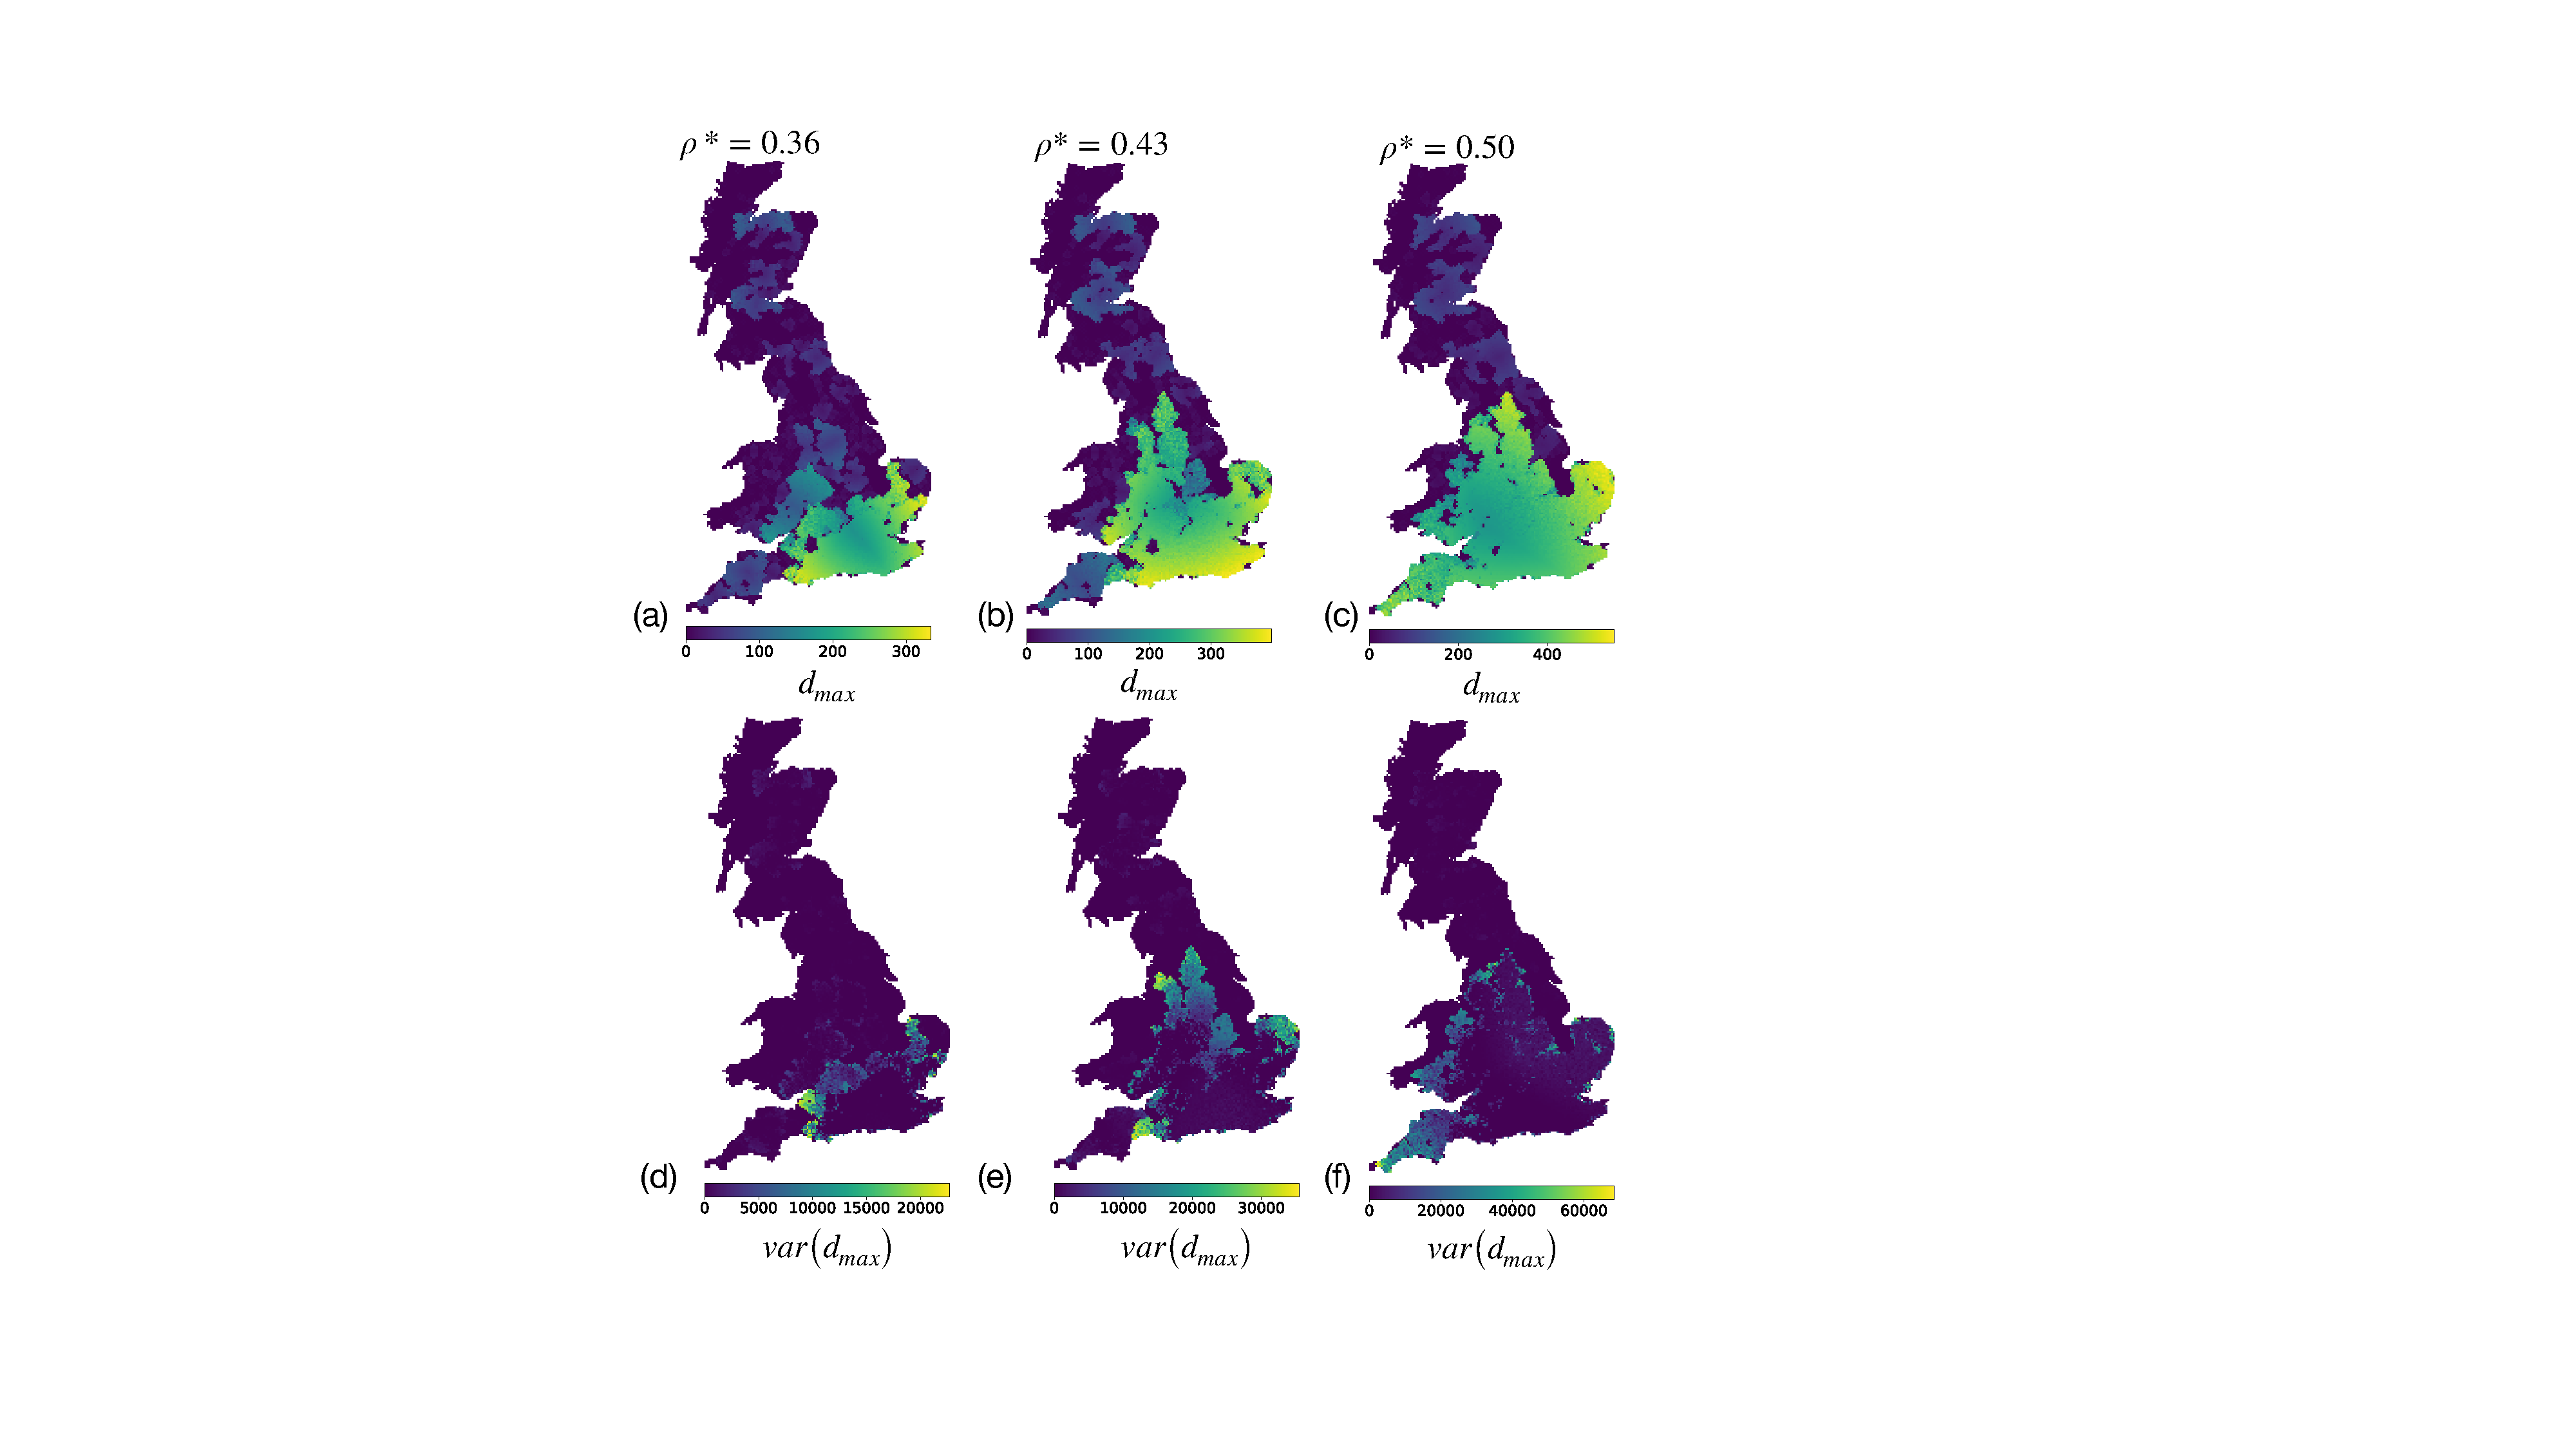
\includegraphics[scale=0.45]{appendix/figures/A-ch4figure1.pdf}
    \caption{Spatial plots showing the pathogens ensemble-averaged maximum distance $d_{max}$ for infectiviy $\beta=0.25$ and density parameters shown.}
    \label{fig:max-distance-metrix}
\end{figure}

\chapter{The non-local dispersal model}
\label{section:apendix_A}

\section{An alternate $R_0$ derivation}
\label{eq:alternate-R0}

Starting from an un-normalised Gaussian kernel $g(p, q; \ell) = \exp(\frac{p^2-q^2}{2\ell^2})$ and infectivity constant $\beta$, we may define the probability of position $q$ being infected due to an infected tree at $p$ as $Pr(q; p) = \beta g(p, q; \ell)$. The domain has tree density $\rho_0$ at time $t=0$ and trees transition through states: $S\rightarrow I\rightarrow R$, with $I$ lasting for $T$ time-steps. Considering the probability of point $q = (x, y)$ becoming infected on account of an infected tree located at the origin during the first time-step:
\begin{equation}
    Pr(x, y, t=0) = \beta \rho_0 \exp(-\frac{x^2+y^2}{2\ell^2})
\end{equation}{}
 Integrating this over an infinite domain gives $R_0(t=0)$ expected infections, given by:
\begin{equation}
    R_0(t = 0) = \beta \rho_0 \int^{\infty}_{-\infty} \exp(-\frac{x^2+y^2}{2\ell^2})dx dy= 2\pi\beta\rho_0\ell^2
\end{equation}{}
At time-step $t+1$ there are less trees to infect. Therefore tree density $\rho$ should also be considered as a monotonically decreasing function of time $\rho(t)$, and the number of expected infections should be given by:
\begin{equation}
    R_0(t) = 2\pi\beta\ell^2\rho(t)
    \label{eq:r0-A}
\end{equation}{}
 Considering density as a function of time\footnote{Density also varies with space as trees are removed quicker for regions closer around the primary infection. However, negating this lead to an easily solvable expression valid for lower-value regimes.} in a discrete domain of size $L$, the average decrease in tree density over one time-step is given by:

\begin{equation}
\label{eq:discrete-rho-t-A}
\begin{split}
\rho(t+1) & = \rho(t) - \frac{R_0(t)}{L^2} \\
 & = \rho(t)\Big(1 - 2\pi\beta\frac{\ell^2}{L^2} \Big)
\end{split}
\end{equation}

at $\rho(t=0)=\rho_0$, therefore, equation (\ref{eq:discrete-rho-t-A}) forms a series from which we may expand to give a continuous equation of $\rho$:
\begin{equation}
    \rho(t) = \rho_0 \big(1 - 2\pi\beta\frac{\ell^2}{L^2}\big)^t
\end{equation}{}
upon substitution back into equation (\ref{eq:r0-A}) we have an approximation for how the number of expected infections from one infected tree is expected to change over time:
\begin{equation}
    R_0(t) = 2\pi\beta\ell^2\rho_0 \big(1 - 2\pi\beta\frac{\ell^2}{L^2} \big)^t
    \label{eq:Rt-A}
\end{equation}{}
This expression is compared against numerical simulations in Fig \ref{fig:sgm-evol}(c). Then integrating over the infectious life-time $t=T$ gives an approximation to an effective reproductive number denoted by $R_0$:

\begin{equation} \label{eq1}
\begin{split}
R_0 & = 2\pi\beta\ell^2\rho_0 \int ^T _0 \big(1 - 2\pi\beta\frac{\ell^2}{L^2} \big)^t dt \\
 & = 2\pi\beta\ell^2\rho_0 \frac{ (1 - 2\pi \beta\frac{\ell^2}{L^2})^T - 1}{\ln(1 - 2\pi\beta\frac{\ell^2}{L^2})}
\end{split}
\end{equation}

(from $\int c^t dt = \frac{c^t}{\ln(c)}$). The expression for $R_0$ can be simplified by noting the pathogen is unlikely to infect trees beyond a distance of $3\ell$, therefore, we can replace the area of the domain with the area over three standard deviations (i.e. $9\pi\ell^2$), thus leading to the approximation:
\begin{align*}
    R_0 = 2\pi\beta\rho_0\ell^2 \frac{(1 - 2/9\beta)^T - 1}{\ln(1-2/9\beta)}
\end{align*}

\section{SIR fitting}

\label{A:sir-fitting}
\begin{figure}
    \centering
    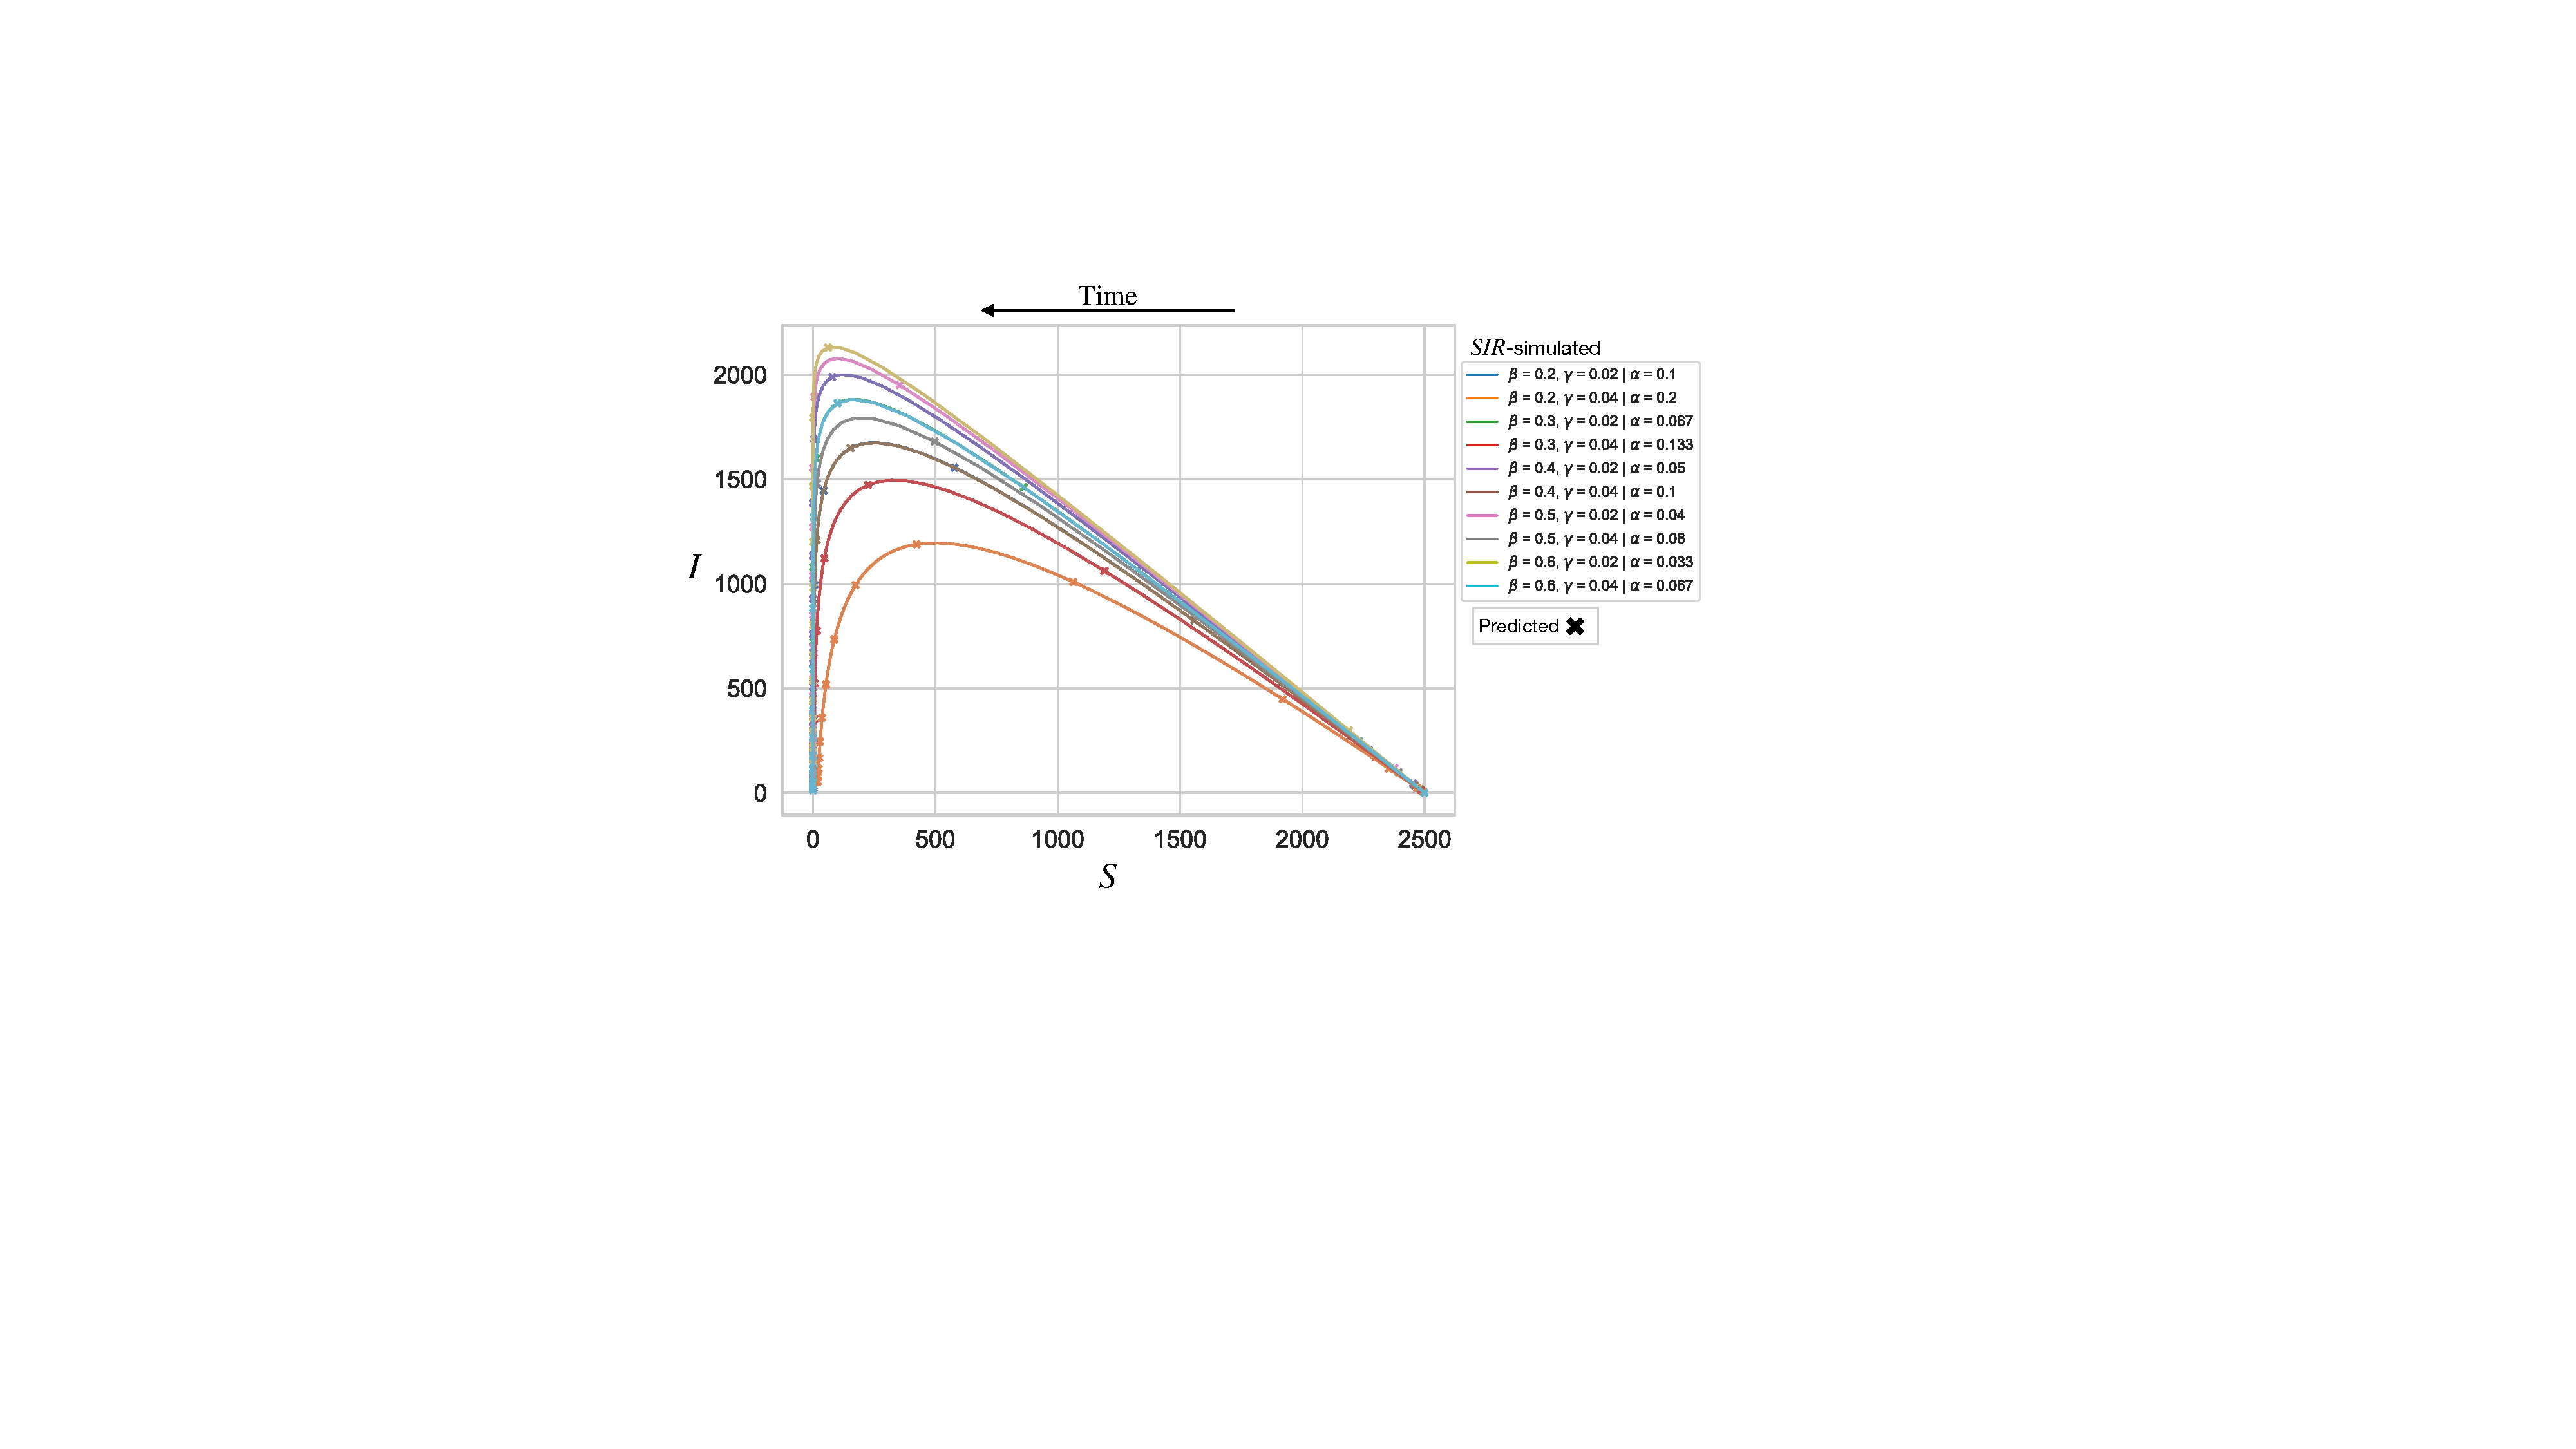
\includegraphics[scale=0.54]{chapter5/figures/fig2-sir-fitting-A.pdf}
    \caption{Infected hosts are plotted as a function hosts, according to the $SIR$ model for various ratios of $\alpha=\gamma / \beta$.
            Initial conditions began from one infected and 2500 susceptible hosts\textemdash equivalent to a $500\times500$ domain at tree density $0.01$.
            Numerical solutions of the $SIR$ model are plotted against predictions from equation \ref{eq:SIR-1param1}, shown as crosses.}
    \label{fig:sir-fitting-a}
\end{figure}

The standard $SIR$ model has no well-known analytic solution, which complicates model fitting.
As such, a simplified scheme that reduced the $SIR$ model to one parameter was used as a comparative tool to access NLM simulations.
Previously in chapter \ref{ch5:dispersal-model}, details were omitted about the behaviour of equation \ref{eq:SIR-1param1}, i.e.
\[
I(S) = -S +  N \Big( 1 + \alpha \ln(S / S_0) \Big)
\]
In Figure \ref{fig:sir-fitting-a}, numerical simulations of the $SIR$ model are compared against analytic predictions from equation \ref{eq:SIR-1param1}.
Specifically, the $SIR$ model was simulated\textemdash using the Euler method\textemdash for various combinations of infectivity rate $\beta$ and removal rate $\gamma$ beginning from
one initially infected and 2500 susceptible hosts.
Numerical $SIR$ simulations and predictions of infected hosts $I$ (from equation \ref{eq:SIR-1param1}) are shown as solid lines and crosses respectively.
As the ratio $\alpha=\gamma/\beta$ decreases, a sharper rise in the infections field $I$ results, indicating a more infectious outbreak.
In contrast, a larger value of $\alpha$ defines a smoother curve which attains a lower peak.
Although equation \ref{eq:SIR-1param1} has clear limitations and descriptive power, it allows a simple one-parameter model to fit the NLM against.


\subsection{Exponentially distributed times}

\label{a:exponentially-distributed-lt}
In Chapter \ref{ch5:dispersal-model}, the NLM was constructed with uniform transitions into the removed compartment.
Here, `uniform' refers to a transition into the $R$ compartment exactly $T$ time-steps after a host becomes infected.
Arguably, uniform life-time transitions are simple and unrealistic.
As such, the NLM constructed in Chapter \ref{ch5:dispersal-model} was re-run with exponentially-distributed life-times. 
Figure \ref{fig:SIR-fitting-expontial} shows the SIR fitting procedure against the exponentially-distributed variant of the NLM. 
Model behaviour in Figure \ref{fig:SIR-fitting-expontial} looks much the same, although fitting the exponentially-distributed NLM to the SIR model resulted in a closer fit for all panels except (b). 
Exponential life-time are implicit within the standard $SIR$ framework\textemdash discussed previously in section \ref{sec:SIR-vs-plank}.
Therefore, it is unsurprising that Figure \ref{fig:SIR-fitting-expontial} generally agrees more with the $SIR$ model, as per equation \ref{eq:SIR-1param1}.
What is surprising is Figure \ref{fig:SIR-fitting-expontial}(b), showing a much larger disparity. 
An explanation of the disparity can be put forward by noting that simulations with fixed, uniform transitions with $T$ lifetimes are typically
more infectious that exponentially-distributed lifetimes with mean $T$. Figure \ref{fig:SIR-fitting-expontial}(b) therefore depict simulations
with lower epidemic severity than the equivalent panel shown in Chapter \ref{ch5:dispersal-model}, Figure \ref{fig:SIR-fitting}(b).
As such, the lower-valued epidemic severity compounds the slowly-spreading wave-like regime (small $\ell$, large $L$) shown in Figure \ref{fig:SIR-fitting}(b).
Consequently, the fitted $SIR$ model shown in red predicts a considerably higher rate of spread.

\begin{figure}
    \centering
    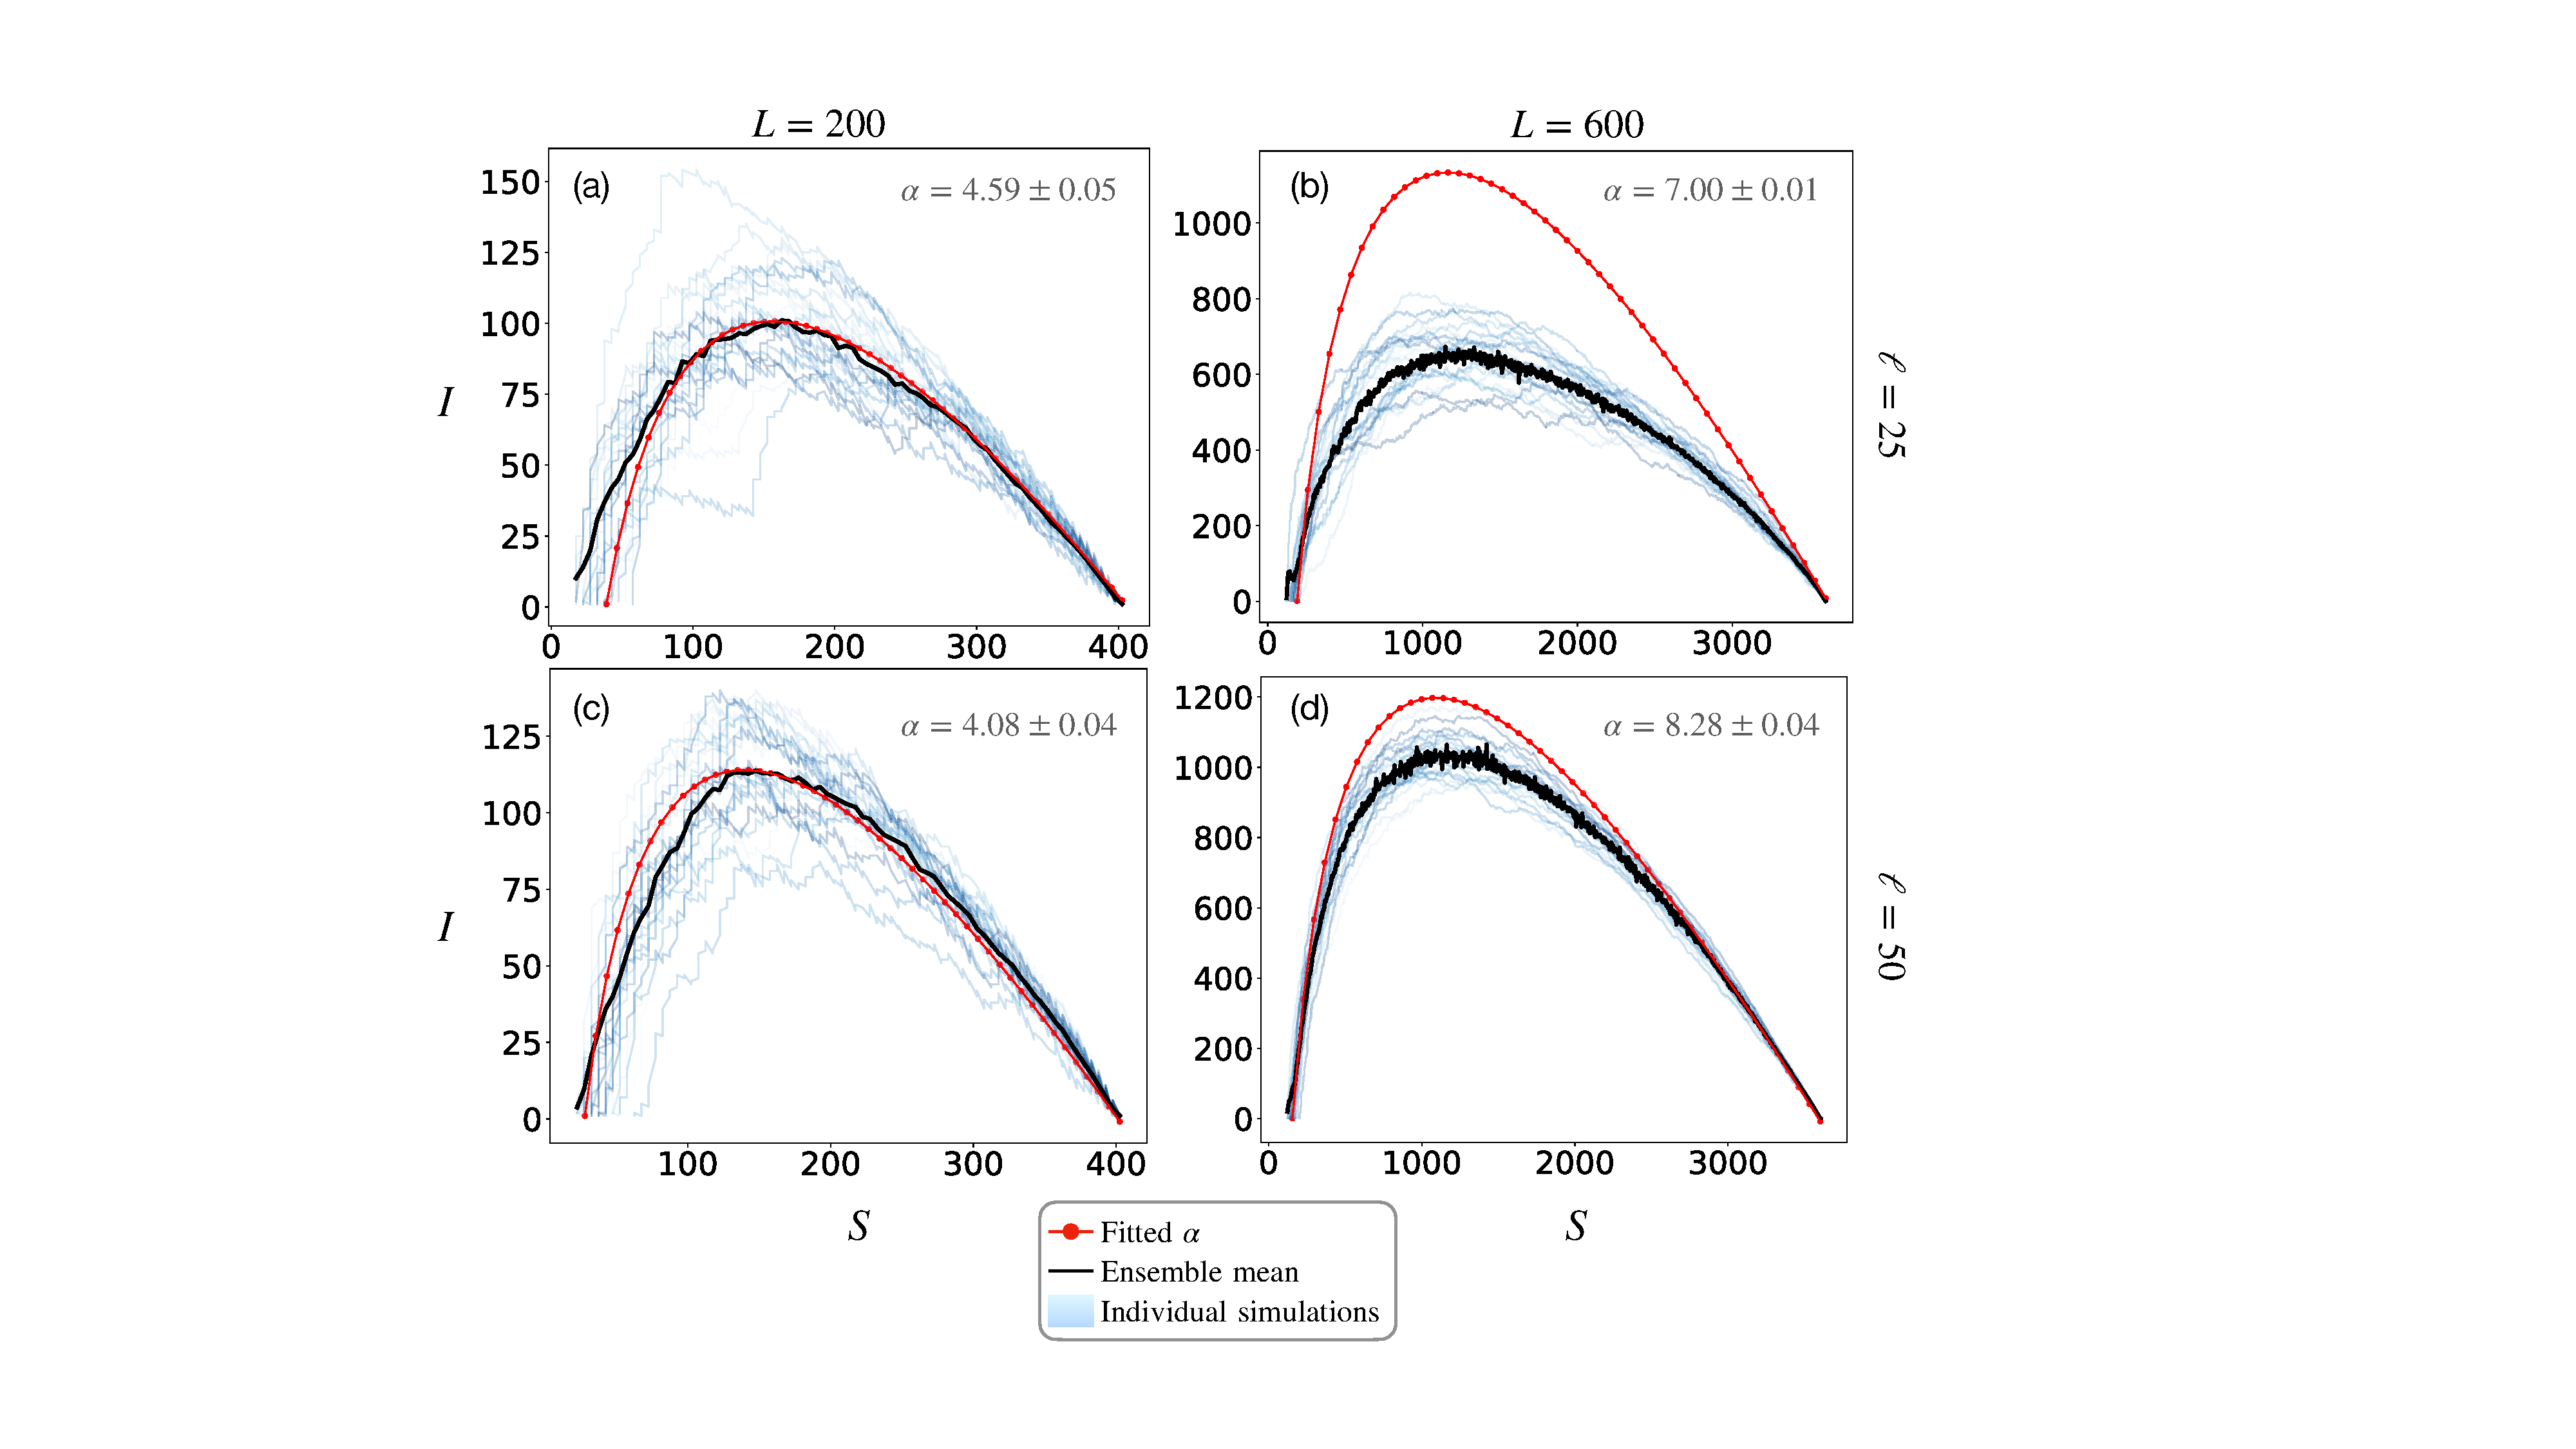
\includegraphics[scale=0.4]{chapter5/figures/fig2-sir-fitting-exp.pdf}
    \caption{Fitting the NLM with exponentially-distributed infectious lifetimes to equation \ref{eq:SIR-1param1}. 
    The equivalent Figure with `uniform' infectious lifetimes was shown in Figure \ref{fig:SIR-fitting}.
    }
    \label{fig:SIR-fitting-expontial}
\end{figure}

\newpage

\section{NLM: probabilistic implementation}
\label{A:combiniing-probabilities}

Infection probabilities in the NLM are statistically independent events.
Suppose that $I_{y1}$ and $I_{y2}$ are two distinct infected trees (where $y1 \neq y2$), and that one susceptible tree $S_x$ at location $x$ exists in the domain.
In this case, $S_x$ will experience infection pressure from $I_{y1}$ and $I_{y2}$.
Assuming that $I_{y1}$ and $I_{y2}$ survive over the time-step $t \rightarrow t + 1$, an infection probability follows the inclusion-exclusion principle:
\begin{equation}
    Pr(S_x \rightarrow I_{x}; I_{y1}, I_{y2}) = P_{y1} + P_{y2} - \big[ P_{y1} \cap P_{yn} \big] 
\end{equation}
where $P_{y1}$ and $P_{y2}$ are the individual probabilities of transition due to $I_{y1}$ and $I_{y2}$ respectively.
In Chapters 5 and 6, these infection probabilities followed Gaussian and inverse power-law dispersal models.
Now, suppose there are $yN$ infected trees, the inclusion-exclusion principle is generalised to give the well-known form:
\begin{equation}
\label{eq:combined-pr}
     Pr(S_x \rightarrow I_{x}; I_{y1}, I_{y2}...I_{yN}) = \sum_{k=1}^{N} \big(  -1 \big)^{k+1} \Big[ \sum _{1\leq y1 \leq y2 \leq....\leq P_{yk} \leq N} \big| P_{y1}\cap ...\cap P_{yk}  \big|   \Big]
\end{equation}
where each intersection $P_{y1} \cap ... \cap P_{yk}$ adds a small order correction to the individual transition probabilities $P_{y1}, P_{y2},..., P_{yN}$.
Equation \ref{eq:combined-pr} is complicated, unsightly and computationally hard to simulate.
Moreover, the definition of $R_0$ becomes more obscure with equation \ref{eq:combined-pr} because secondary can in principle be induced under the influence of multiple sources.

Nevertheless, equation \ref{eq:combined-pr} can be significantly simplified. 
Consider once again the system of two infected trees ($I_{y1}$ and $I_{y2}$) and one susceptible ($S_x$).
The probability of $S_x$ remaining unaffected is given by:
\begin{equation}
    Pr(S_x \rightarrow S_{x}; I_{y1}, I_{y2}) = (1 - P_{y1})(1 -P_{y2})
\end{equation}
and now the probability of $S_x$ becoming infected is:
\begin{equation}
\label{eq:pr-simp}
    Pr(S_x \rightarrow I_{x}; I_{y1}, I_{y2}) = 1 - Pr(S_x \rightarrow I_{x}; I_{y1}, I_{y2})
\end{equation}

Generalising equation \ref{eq:pr-simp} to a system of $N$ infected trees and $M$ susceptible trees, over a single time-step we have:
\begin{equation} \label{eq-full-pr}
\begin{split}
Pr(S_{x1} \rightarrow I_{x1}) & = 1 - \prod_{n=1}^{N}(1 - P_{yn})\\
&\vdots \\
Pr(S_{xM} \rightarrow I_{xM}) & = 1 - \prod_{n=1}^{N}(1 - P_{yn})
\end{split}
\end{equation}
where the repeated product is introduced for brevity, and multiples each transition probability, i.e $(1 - P_{y1})(1 - P_{y2})  \hdots (1 - P_{yN})$. 

In pseudo-code, equations \ref{eq-full-pr} follow:
\begin{lstlisting}[style=pythoncode,
    caption = ,
    label = py:rand]
                # IMPLEMENTATION (A): Full inclusion-exclusion
def run_algorithm(S_tree_arr, I_tree_arr, R_tree_arr, run_times):
    
    for time_step in range(run_times): # iterate over time-steps
        for S_i in S_tree_arr:  # iterate over susceptible trees 
            for I_j in I_tree_arr:
                # iterate & store individual probabilities
                Pr(S_i --> I_i; I_j) 
            # combine all probabilities as in equation B.12
            Pr(S_i --> I_i; I_1,I_2,..., I_N)
            update I_tree_arr # updated infected tree arr
            update R_tree_arr # update removed tree arr
            if BCDs:
                end
\end{lstlisting}
However, upon simulation, it was noted that each individual probability ($P_{y1}...P_{yN}$) is small.
Otherwise, the degree of epidemic spread becomes unphysical\textemdash consider the limiting behaviour when a single infected tree infects every susceptible in one time-step. 
For the epidemic parameters of interest, it was noted that combining all probabilities with the inclusion-exclusion principle (as per the system of equations \ref{eq-full-pr}) was unnecessary
because small-order corrections (intersection $P_{y1} \cap ... \cap P_{yk}$) become trivially small. 

A simpler, more intuitive implementation that neglects the probability intersections can be put forward as:
\begin{lstlisting}[style=pythoncode,
    caption = ,
    label = py:rand]
                # IMPLEMENTATION (B): Approx inclusion-exclusion
def run_algorithm(S_tree_arr, I_tree_arr, R_tree_arr, run_times):
    
    for time_step in range(run_times): # iterate over time-steps
        for I_i in I_tree_arr:  # iterate over infected trees 
            for S_j in S_tree_arr:
                # compute individual probabilities
                Pr(S_j --> I_j; I_i) 
                update I_tree_arr # updated infected tree arr
                update R_tree_arr # update removed tree arr
                if BCDs:
                    end
\end{lstlisting}
here, we iterate over \textit{infected} trees rather than susceptible trees. 
In this scheme, individual probabilities between infected and susceptible trees are computed sequentially.
Henceforth, both schemes are denoted as `implementation' (A) and (B), i.e. full and approximated inclusion-exclusion formulas respectively.

\subsection{Contrasting implementations: epidemic spread}

Implementations (A) and (B) are compared in Figure \ref{fig:imp-comp}. 
Plots in Figure \ref{fig:imp-comp} show the number of removed trees in $R$, or tree mortality, for two values of dispersal $\ell=25$ and $\ell=50$ and three values of infectivity.
In each panel, $25$ ensemble realisations were computed, and both tree density and domain size are fixed to $\rho=0.01$, $L=350$, respectively.
Overall, both implementations give rise to the same epidemic, illustrated by the similarity between orange and blue plots.

\begin{figure}
    \centering
    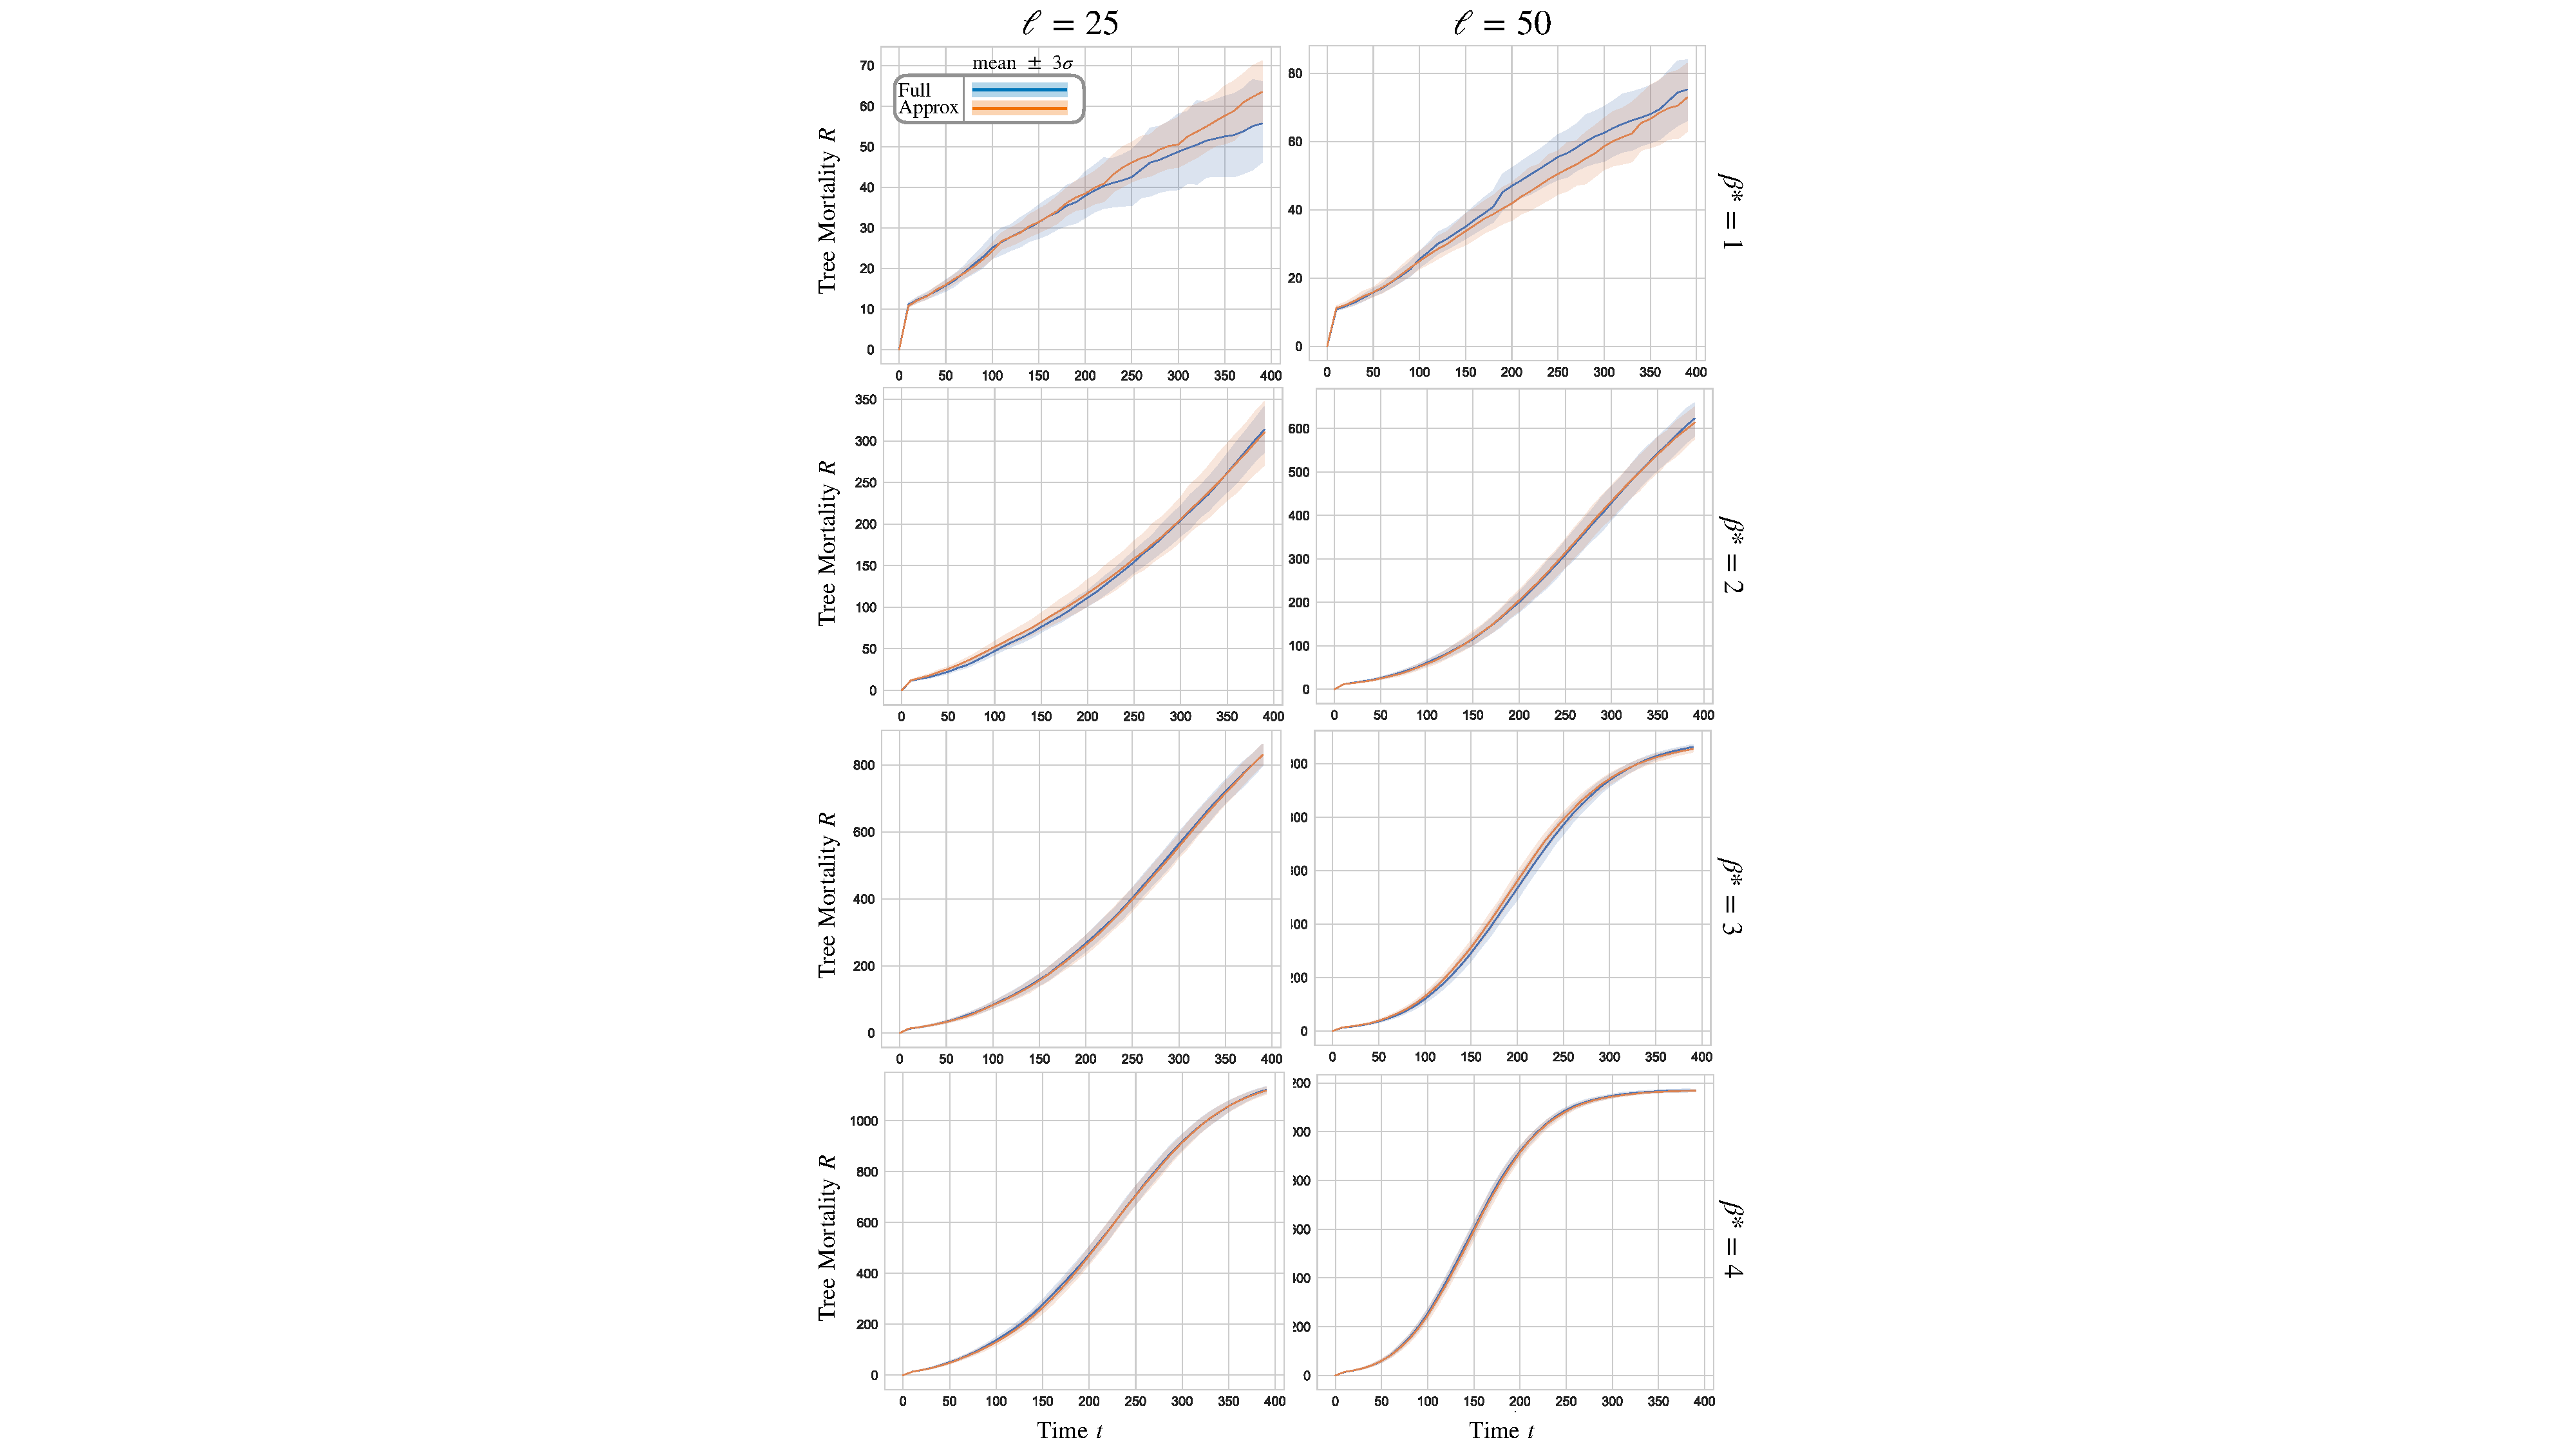
\includegraphics[scale=0.60]{chapter5/figures/appendix-implementation.pdf}
    \caption{Comparing both the approximated and full probability implementation methods reveals little to no differences in the tree mortality, or number of removed trees $R$, over time for different epidemic parameter combinations. All plots show $\rho=0.01$, $L=350$, and were seeded by ten initally infected trees. }
    \label{fig:imp-comp}
\end{figure}

Two values of dispersal were contrasted, motivated by the idea that for a larger dispersal value, the intersections of ($P_{y1}...P_{yN}$) might be larger as trees can interact further apart.
Although, no divergence can be seen between $\ell$ values in Figure \ref{fig:imp-comp}, except for a slightly more infectious system when $\ell=50$\textemdash consistent with the results shown in Figure \ref{fig:R0-analytic-vs-sims}(c).
Indeed, even highly infectious epidemic systems with $\beta^*=25$ and $\beta^*=100$ ($10 \lessapprox R_0 \lessapprox 100$) the spread of disease remains the same. 
Simulations therefore indicate that for physical epidemic regimes, both implementations are virtually identical. 
At some parameter values, neglecting the intersections $P_{y1} \cap ... \cap P_{yk}$ would undoubtedly deviate from the full inclusion-exclusion formula. 
However, we have not encountered a realistic epidemic regime were the approximation becomes inaccurate 
throughout this thesis.

\subsection{Contrasting implementations: computational cost}

Despite epidemic simulations remaining the same, a large difference was noted in the computational cost (and runtime) between both implementations.
Figure \ref{fig:imp-runtime} contrasts the computer runtime (in seconds) over a range of infectivity parameters and two tree densities.
Both panels (a) and (b) depict a system with $\ell=50$ and $L=500$ over $10$ ensemble realisations. 
Interestingly, the full inclusion-exclusion formula, as per implementation (A), is more efficient when $\beta^*$ is large and the number of infected trees is high.
Whereas, the approximated inclusion-exclusion formula, as per implementation (B), is more efficient when $\beta^*$ is low and the number of infected trees is small.

The trends in Figure \ref{fig:imp-runtime} can be understood by realising that when infectivity is high, the number of infected trees grows quickly. 
A large number of computations arise in implementation (A) for lower values of $\beta^*$, as we iterate through a large number susceptible trees.
Consequently, the runtime is large, particularly when the infection spreads slowly and the number of trees in $S$ remains relatively large throughout the simulation.
As $\beta^*$ is increased, the number of trees in $S$ decrease rapidly, and runtime decreases accordingly. 
The situation is similar for implementation (B). 
When $\beta^*$ is high, a larger number of infected trees entails a larger number of computations as we primarily iterate over the infected trees.

\begin{figure}
    \centering
    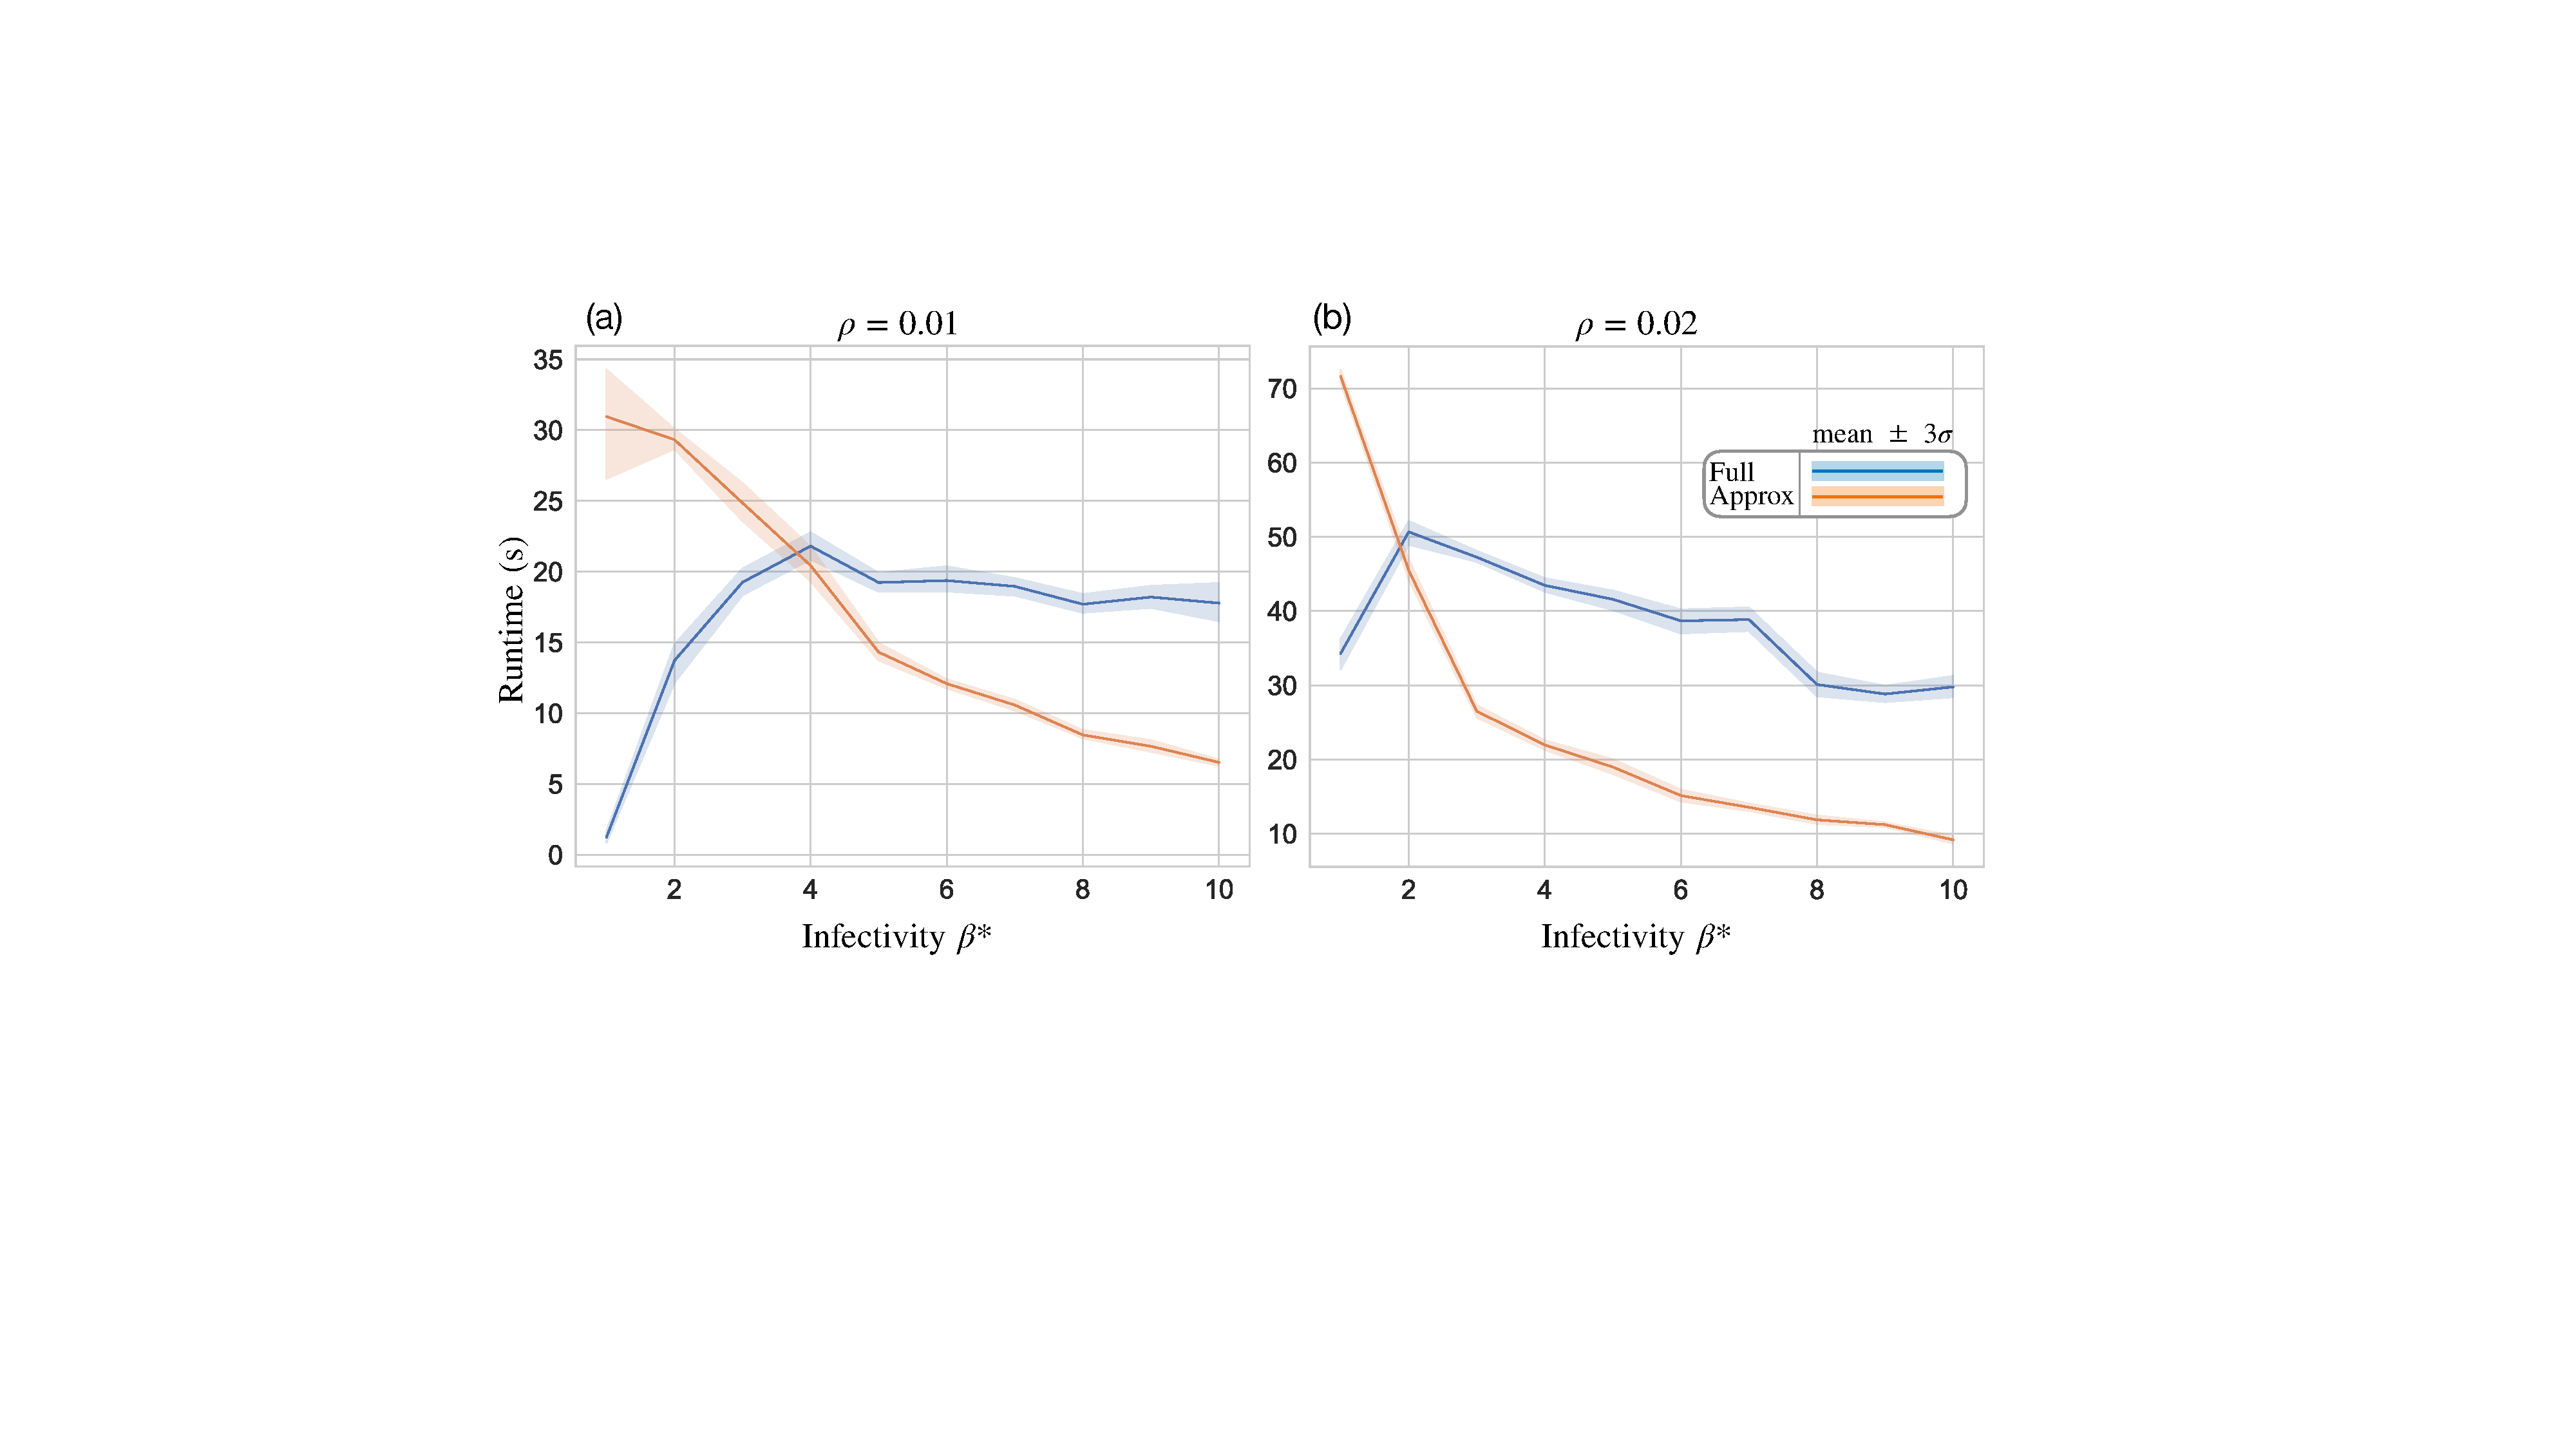
\includegraphics[scale=0.425]{appendix/figures/runtime-comp.pdf}
    \caption{A comparative look at the difference between simulation runtime (in seconds) between both probability implementations.
    When the number of infected trees is small for low $\beta^*$, the approximated scheme (implementation B) is more efficient and runs quicker. 
    In contrast, when the number of infected trees is high for large $\beta^*$, full inclusion-exclusion formula (implementation A) becomes more efficient.
    Overall, the simulation runtime increases with the tree density.
    }
    \label{fig:imp-runtime}
\end{figure}

Given the virtually identical spread between both implementation methods (A) and (B), it is alluring to remark about the possibility of switching between implementation (A) for lower and (B) for severe epidemic regimes, as this has the lowest overall runtime and highest computational efficiency. 
Nevertheless, implementation (B) was chosen throughout the thesis because it is more intuitive and efficient for the epidemic regime we are interested in, typically around the average density of trees in GB and $R_0 < 10$.

\subsection{Codebase}

Throughout this thesis, I gravitated heavily toward the software engineering side of the project. 
As such, a single unified codebase can by found at: \nolinkurl{https://github.com/John-Holden/tree_epi_dispersal.git}.
In the repository, an epidemic simulator comprising both the NLM and the seasonal $SEIR$ model of ADB can be found and downloaded.
I took the approach of developing a flexible, integrated codebase, where the user defines what model is run based on configuration option.
In particular, the model configuration is defined by:
\begin{itemize}
    \item which compartments $S$, $E$, $I$, or $R$ are to be run
    \item the domain size $(L_x, L_y)$
    \item the type of dispersal function: Gaussian/exponential/Inverse power law
    \item the type of sporulation function: $\phi_0(t) = 1 \ \forall t$ (Ch 5), $\phi_1(t)$, $\phi_2(t)$ (Ch 6,7)
    \item epidemic parameters, density, infectivity and dispersal $(\rho, \beta, \ell)$
    \item infection life-times: uniform/exponential dynamics, $T$ steps
    \item which metrics are to be collected, e.g. time series, $R_0$, tree mortality, spread velocity
    \item initial and boundary conditions, e.g. end simulation when all infectives die 
    \item ensemble realisations: iterate a user-defined function $N$ times and store
    \item whether or not simulations are run on a HPC (Leeds arc3) or the local machine
\end{itemize}

\section{Contact-tracing $R_0$}
\label{A:R0-contact-traced-mortality}

\begin{figure}
    \centering
    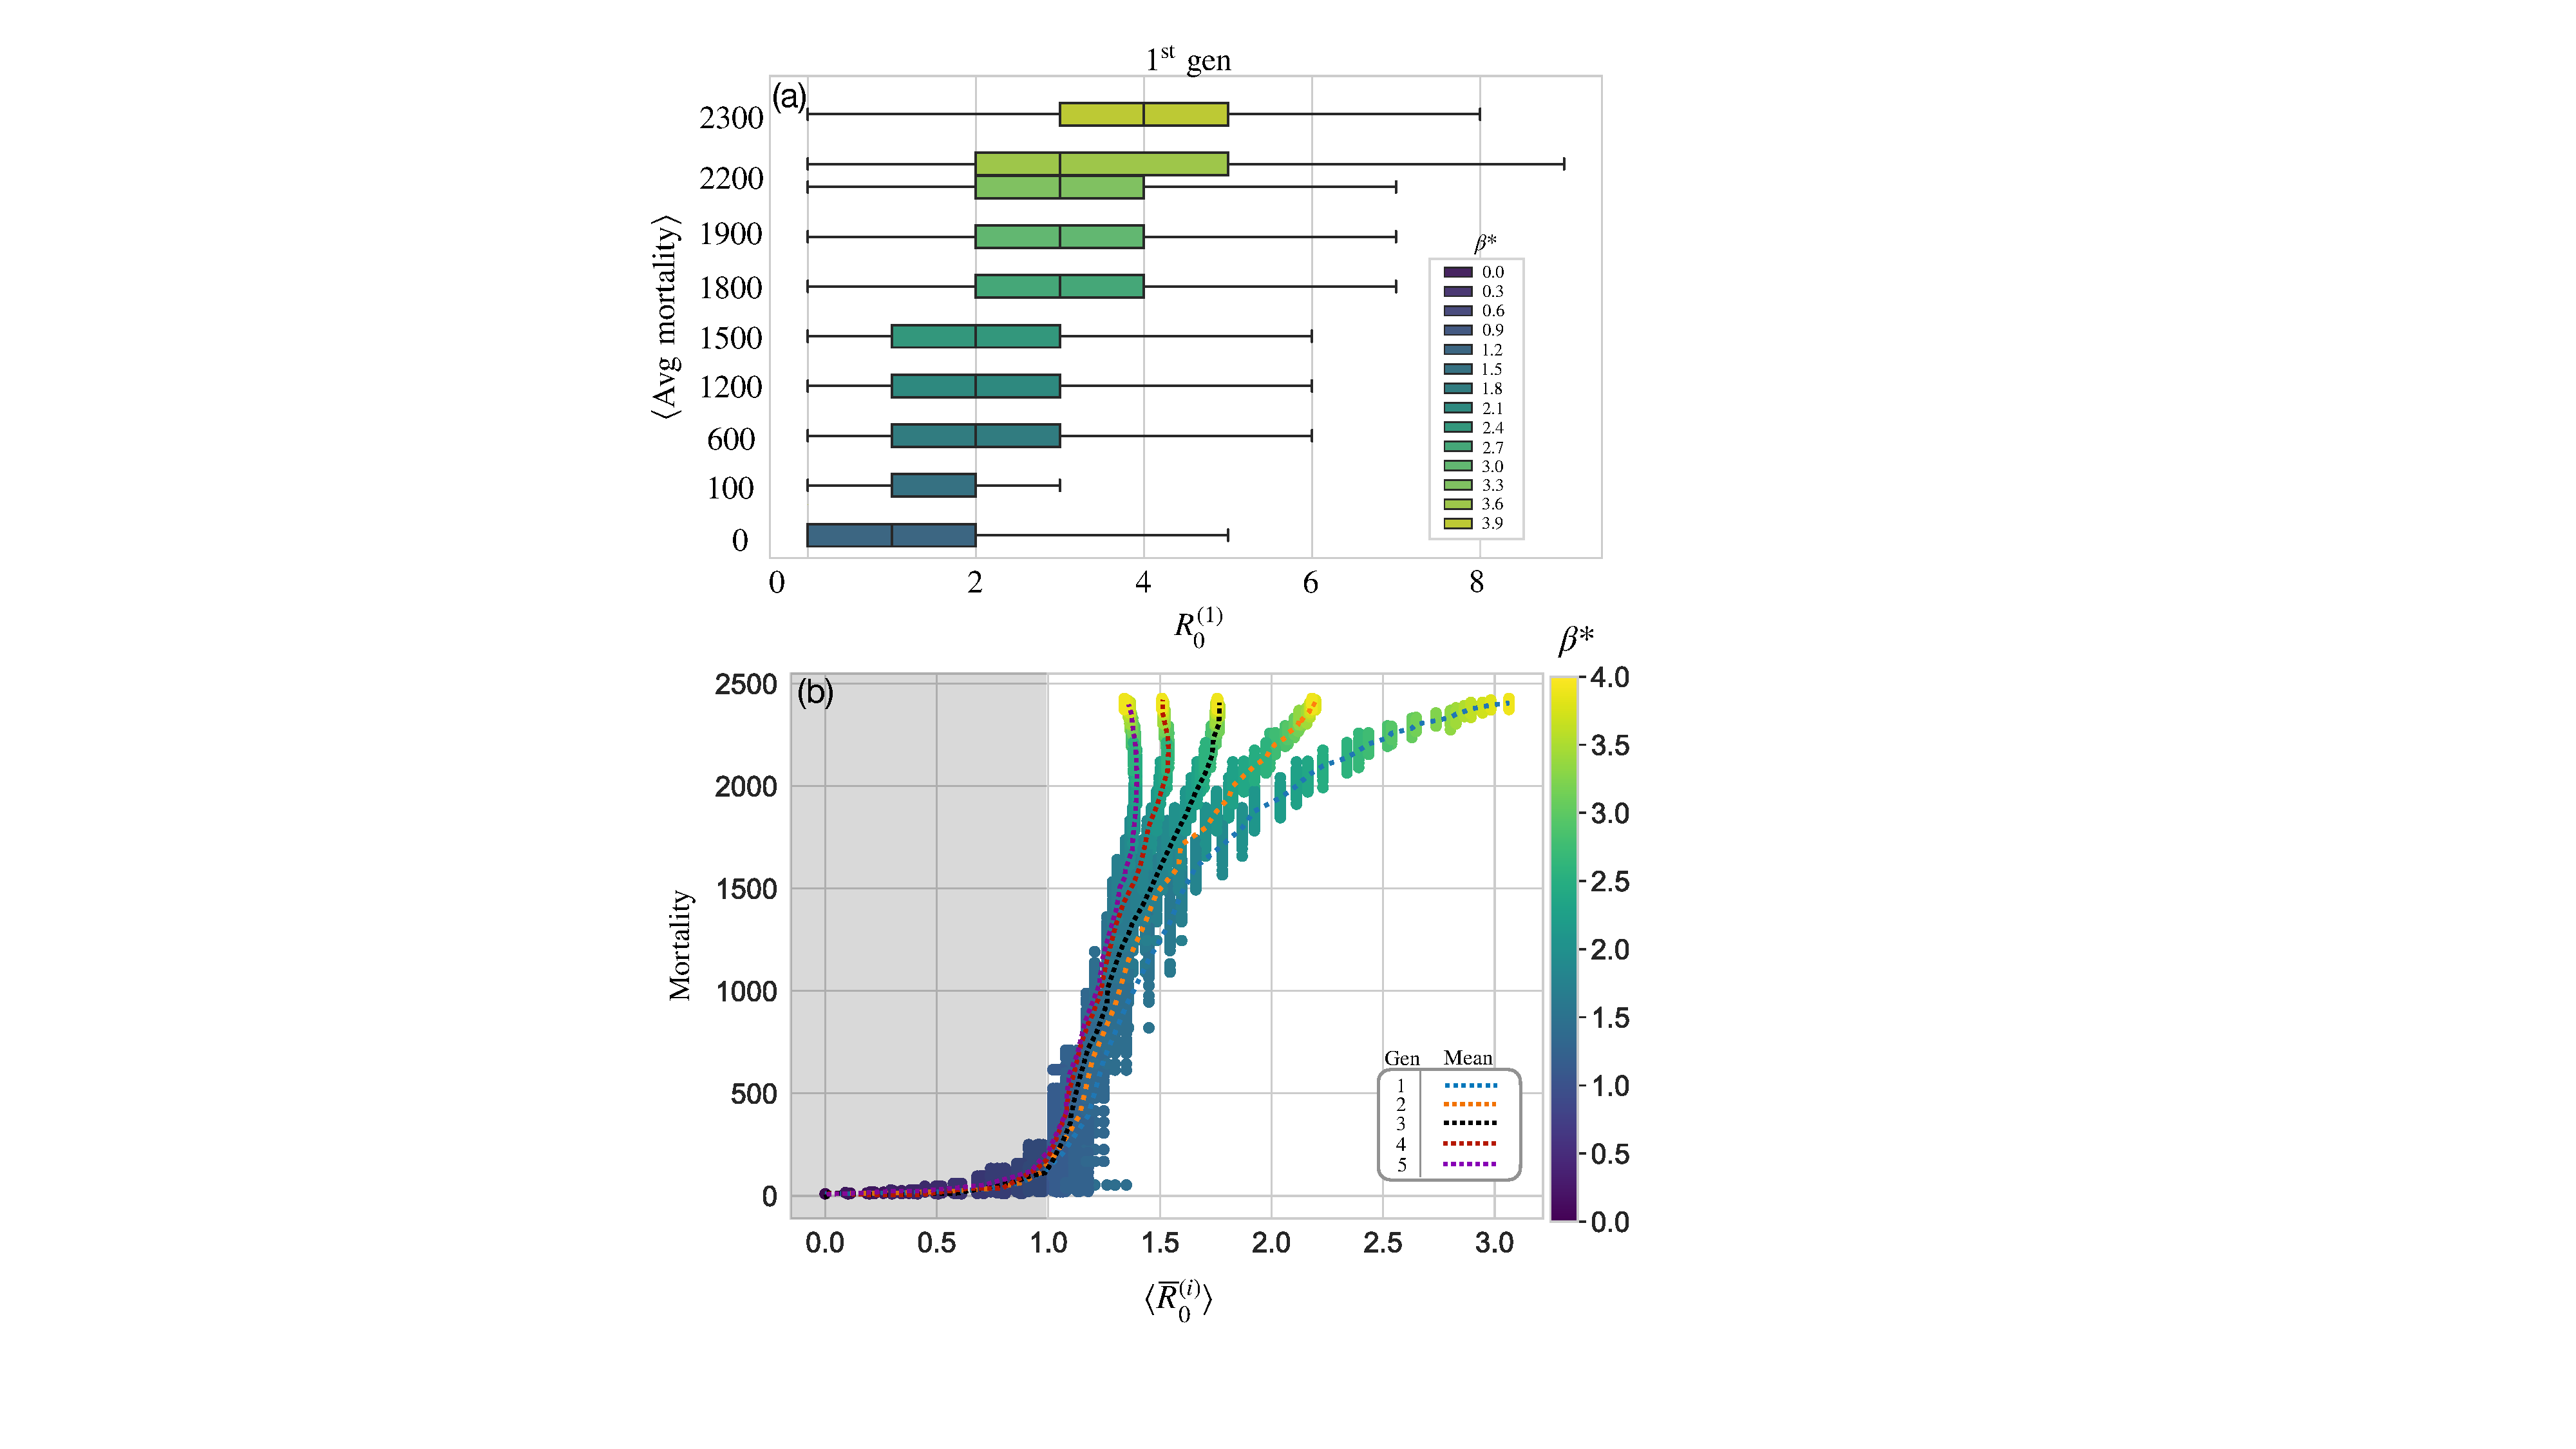
\includegraphics[scale=0.60]{chapter5/figures/fig6-R0-contact-vs-mortality-A.pdf}
    \caption{Comparing the contact-traced reproduction ratio against tree mortality. (a) Inverting the plot of Figure \ref{fig:contact-trace-vs-mortality} to show the spread of $R_0^{(1)}$ against the ensemble averaged tree mortality. (b)
    Re-running the ensemble shown in Figure \ref{fig:contact-trace-vs-mortality} with $10$ initially infected trees. The threshold appears more abrupt and stochasticity is reduced.}
    \label{fig:R0-contact-vs-morality-A}
\end{figure}

In Figure \ref{fig:R0-contact-vs-morality-A}(a), we invert the plot (shown in Figure \ref{fig:contact-trace-vs-mortality}) and show the range of first generation reproduction ratios $R_0^{(i1)}$ against the ensemble-averaged tree mortality.
Inverting the plot gives information about the spread of $R_0^{(1)}$;
as we can see, low values of infectiviy produce a skewed distribution which becomes more centered as infectivity increases.
A threshold can be seen around $R_0^{(1)}=1$, although a number of simulations can produce a low-valued $R_0^{(1)}$ for any value of infectivity due to initial extinction events.
In Chapter \ref{ch5:dispersal-model} both the contact and analytic values of $R_0$ were computed/observed for a single infectious tree at the domain center.
As elaborated in chapter \ref{ch5:dispersal-model}, initial stochastic forces had the tendency to reduce the chance of epidemic by causing early extinction events\textemdash thereby reducing the mean tree mortality.
However, a number of initial conditions are possible.
As such, the plot of Figure \ref{fig:contact-trace-vs-mortality} was re-run with $10$ infectious trees in the domain center at $t=0$ to test how initial stochasticity in the system changes, shown by Figure \ref{fig:R0-contact-vs-morality-A}(b).
As expected, increasing the number of infected trees at $t=0$ reduces stochastic and early extinction events;
this is demonstrated by noting that Figure \ref{fig:R0-contact-vs-morality-A}(b) has a smoother ensemble mean, and no instances of zero mortality for highly infectious epidemics (c.f. the bottom right hand side of Figure \ref{fig:contact-trace-vs-mortality} where multiple observations can be seen of zero tree mortality for high $\beta^*$).
Surprisingly, for later generations the degree of inflexion for $R_0^{(4)}$-$R_0^{(5)}$ is reduced at high $\beta^*$ in comparison to Figure \ref{fig:contact-trace-vs-mortality}.

\newpage

\chapter{Constructing $R_0$-maps and landscape control}

\label{section:ga-SEIR-variant}

\section{Connected component analysis}
\label{a:CCA}

A cluster labelling algorithm was employed to identify and distinguish different clusters of susceptible ($R_0 > 1$) patches in GB.
In Python, the function `label' (in the SciPy library) can be used to identify and label different connected clusters.
Label requires two pieces of information, the object/image to be analysed and the type of connectivity.
Here, we use a 4-connectedness structuring element comprising either Von Neumann or Moore neighbourhoods.
The object/image needs to be in the form of a binary matrix to be analysed;
this requirement fulfilled through the (Bernoulli trial) tree density implementation, composed of either occupied (1) and unoccupied (0) tree states.

The label function performs the following steps to find the connected sites within the binary matrix:
\begin{enumerate}
    \item Search for the next unlabelled site, i.
    \item Perform a flood-fill algorithm to label all the sites connected to site i.
    \item Repeat steps 1 and 2 until all sites are labelled.
\end{enumerate}

\begin{figure}
    \centering
    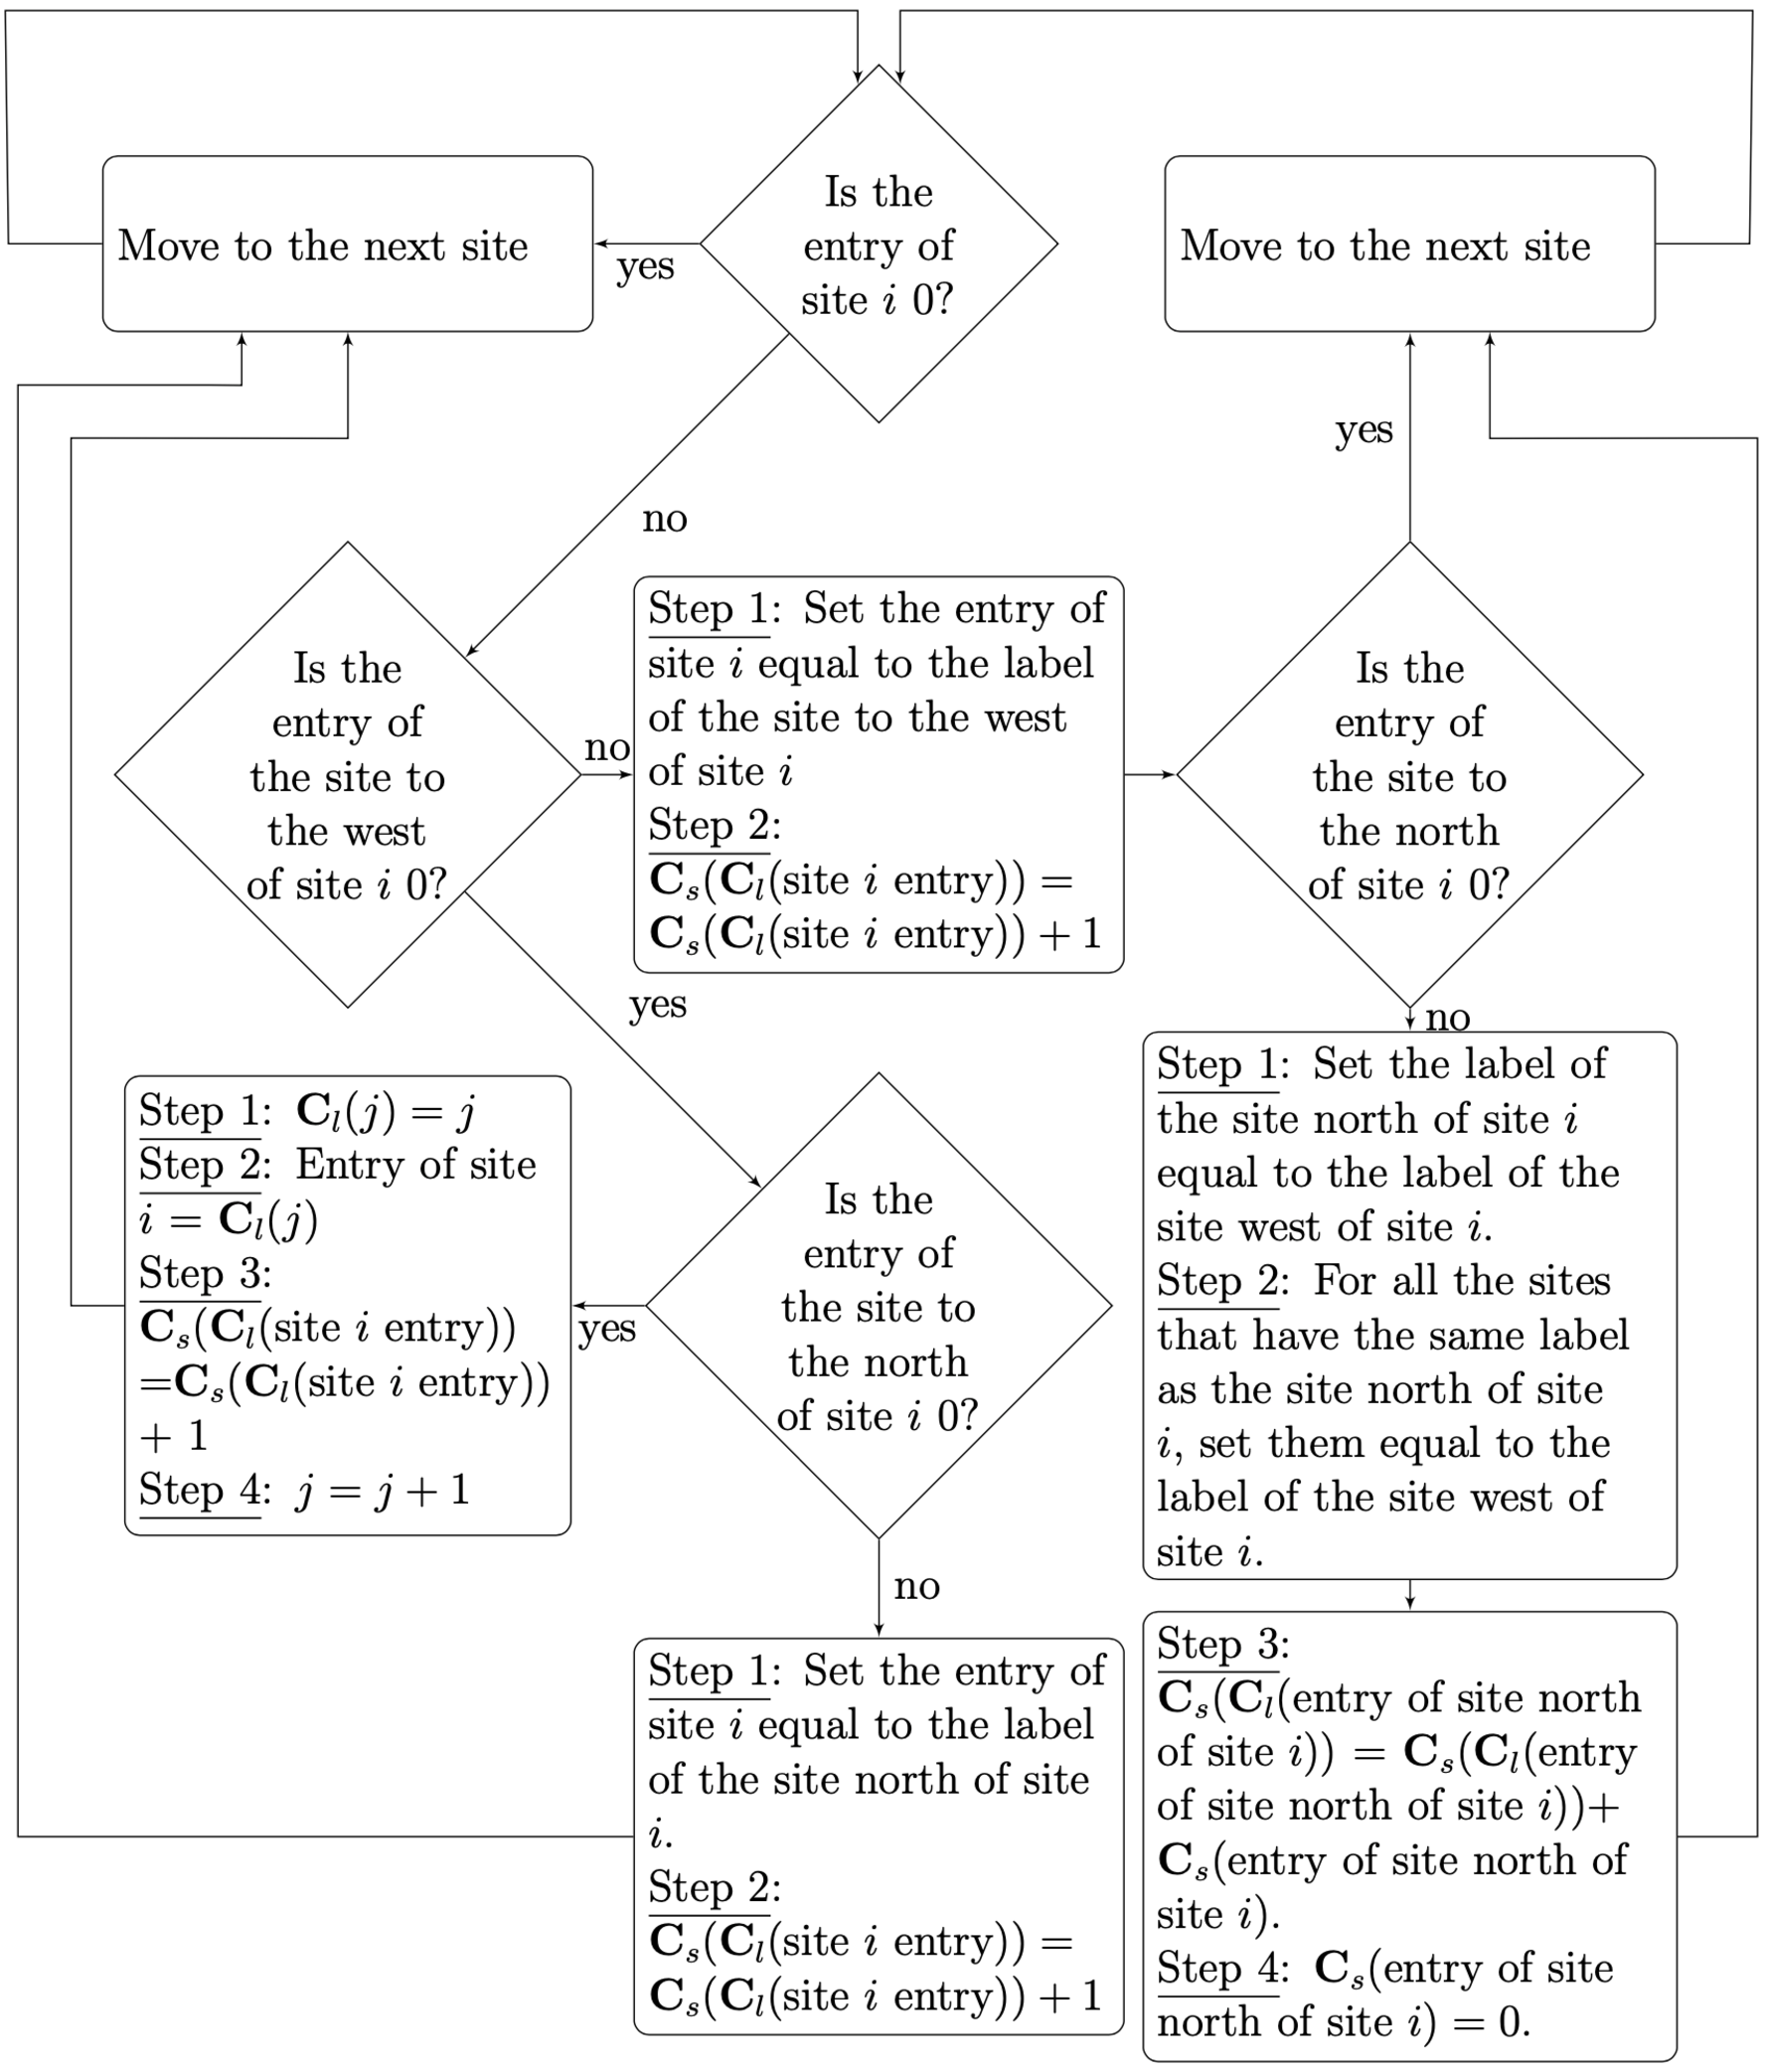
\includegraphics[scale=0.55]{appendix/figures/CCA-Flow.pdf}
    \caption{Flowchart describing the cluster labelling algorithm.}
    \label{fig:my_label}
\end{figure}

The algorithm returns a new structure reflecting the structuring element, 
the image dimension, the number of distinct clusters found, and the size of each cluster. 
Hence, a new matrix with labelled clusters is formed, along with a new variable detailing the cluster sizes. 
The net result is a new image showing each cluster labelled by a unique integer. 
Through this, all of the sites contained within this cluster have the same unique integer label.

First, the algorithm starts the sweep from the top left-most column then iteratively repeats column-by-column. 
Two preliminary variables are created to store: A) the number of clusters in the system and B) the size of each cluster found. 
Both variables are displayed in the output, as separate one-dimensional arrays, denoted by $C_s$ and $C_l$ representing the cluster sizes and the cluster numbers respectively. 
Using these two variables and the occupancy of sites, the methodology of the algorithm is described in the flowchart shown in Figure 3.1.

Both $\mathbf{C_s}$ and $\mathbf{C_l}$ are an essential part of the process, though they are used in fundamentally different ways.
That is, $\mathbf{C_l}$ is used to label each occupied site using the following method:
\begin{itemize}
    \item An index is set to $1$ at the beginning of the algorithm\textemdash and increases by 1 upon finding a new cluster.
    \item If both sites north and west of an occupied site $i$ are unoccupied, site $i$ is given the current index of $\mathbf{C_l}$.
    \item If the site to the north OR the west of the occupied site i are occupied, the site $i$ is assigned the label of the occupied site.
    \item If both sites to the north and west of the occupied site i are occupied, then site $i$ and the site to north of site 
    $i$ are both assigned the label of the site to the west of site $i$.
\end{itemize}

From $\mathbf{C_l}$, the label $j$ $(j = 1,2,3,...)$ of each site can be found through satisfying $\mathbf{C_l}(j) = j$.
The label for each site i that will be stored in $\mathbf{C_l}$ is identified using the following argument:
first, let the original entry of site $(i - 1)$ be $j_1$ and the label assigned to site $(i − 1)$ be $j_2$. 
Then, for site $i$, the following values can be assigned: $\mathbf{C_l}(j1) = j_2 and \mathbf{C_l}(j2) = j_2$, 
resulting in $j_2$ being stored as the label for site $i$. 
Having established the notion of  $\mathbf{C_l}$, the uses of $\mathbf{C_s}$ will now be explored.

The parameter $\mathbf{C_s}$ is used to store the different cluster sizes. 
Whenever an occupied site is assigned a label, 
the corresponding entry of $C_s$ is increased by one. 
When both the sites to the north and west of site $i$ are occupied but have different labels, 
it is necessary to merge the two clusters together and ensure all sites have identical labels. 
The cluster size that has the same label as the entry of the site to the north of $i$ is added to the size of the cluster that has the same label as the site to the west of $i$. 
The size of the cluster corresponding to the site north of $i$ is then zeroed out. 
Repeating this method allows the algorithm to perform a complete sweep. 
This provides an accurate labelling of all occupied sites and the size of all the clusters too. Due to this, only one sweep of the
algorithm is necessary \cite{hoshen1976percolation}.

Using the label function creates an efficient way of labelling multiple clusters relatively quickly.
The output of the algorithm produces easily distinguishable clusters whilst providing data that can be analysed further in a variety of ways. 
This demonstrates the importance of a cluster multiple labelling algorithm (or connected component labelling technique) within many applications, 
be this in percolation theory or other areas of research. 
One of the main complications of using this method is the computational cost that accompanies it. 
We will now go on to explore how this has affected choosing the size of the system to analyse.

% \subsection{CCA Computation cost}

% Cluster multiple labelling techniques are computationally expensive to operate. The com- pletion time of this algorithm is commonly found to be critical in the feasibility of a given algorithm. The algorithm, discussed in more detail in Section 3.2.1, works by assigning a label to an occupied site and attempting to propagate the label to the site’s east and south neighbours [11]. The time taken to perform a full sweep varies dependent on the size of the system, denoted by L, number of clusters and the size of clusters found in the system. Note that the latter two directly depend on the value of p. To demonstrate the effect of changing these two factors (i.e. size and p), the time taken for the foundation code to run has been measured and recorded in Table 3.1. These measurements were obtained using the same machine, as the results are deterministic of the machine used. This provides a realistic representation of how the time scales as the system size, L, is increased. The foundation code consists of the following steps: assigning a matrix size, generating the matrix, and applying the occupation probability p, running the bwconncomp function, creating the labelled cluster matrix and extracting the cluster size information from the output.

\newpage

\subsection{Binary dilation}
\label{sec:a-binary-dialator}

A binary dilator was used to help identify when two distinct clusters ($\mathbf{C_1}$ and $\mathbf{C_2}$) connect.
Suppose a we have a binary image in Euclidean space, $\mathbb{R^2}$.
For our purpose, $\mathbb{R^2}$ consists of susceptible and insusceptible patches, where $R_0 \ge 1$ and $R_0 < 1$ receptively. 
The binary dilator operation is defined by:
\begin{equation}
    \label{eq:binary-dialation}
    A \oplus B = \bigcup_{b \in B} A_b
\end{equation}
where $A_b$ has underdone a translation by the structuring element $b$.
The meaning of equation \ref{eq:binary-dialation} is best described an example:
\begin{figure}[h!]
    \centering
    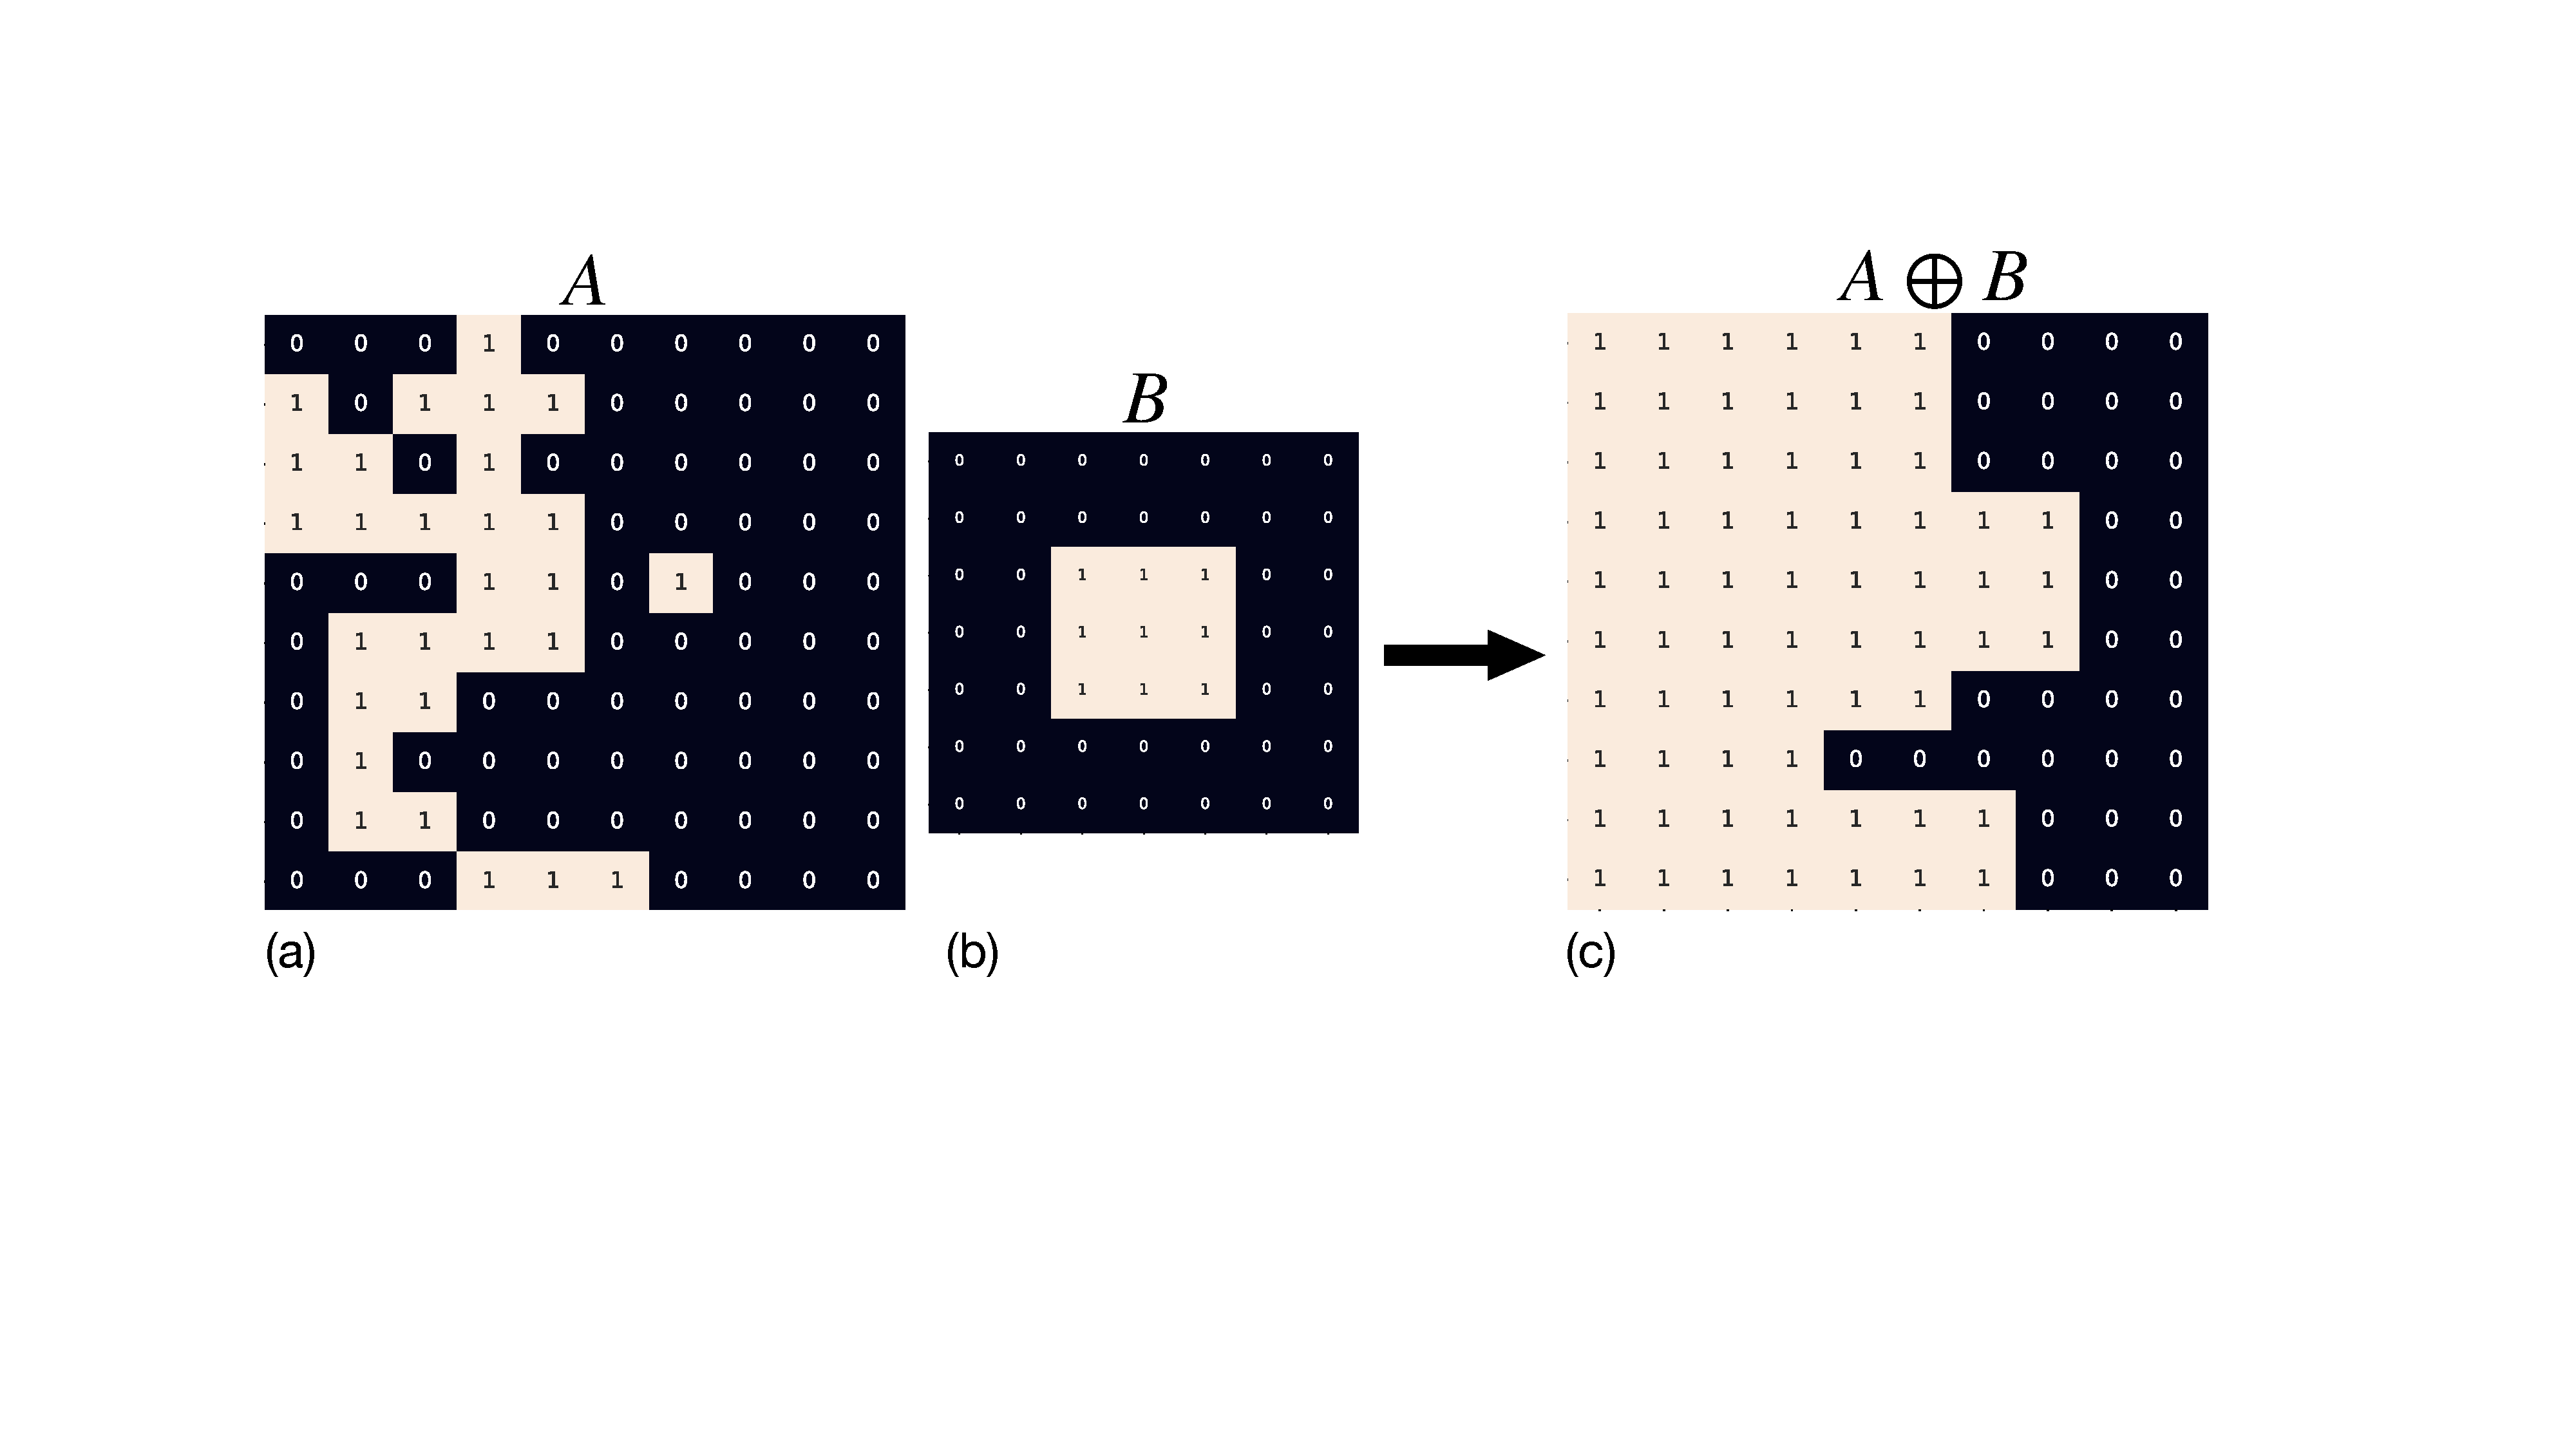
\includegraphics[scale=0.3]{appendix/figures/binary-dialation.pdf}
    \label{fig:my_label}
\end{figure}

here, $A$ is the binary-valued input image and $B$ is the structuring element, in this case, a Moore neighbourhood. 
Then, $B$ is super imposed onto every non-zero value in $A$, thereby forming the binary dilation shown in Figure (c).
Binary dilation was implemented in Python, using the `binary dilation' function within the Scipy.ndimage module \cite{scipy}.

In section \ref{sec:fragmentation-method}, I put forward the first steps toward an algorithm to optimise cluster fragmentation.
In this method, distinct clusters ($\mathbf{C_1}$ and $\mathbf{C_2}$) connected for some value of $\xi$.
Detecting cluster joins turned out to be non-trivial problem to solve.
The naive approach would be to perform a brute-force search, and detect which connecting patches bridge the gap between $\mathbf{C_1}$ and $\mathbf{C_2}$
for each step in $\xi$. 
However, this approach quickly became computationally hard to solve, particularly when $\xi$ was low and the number of susceptible patches in the system was large. 
\begin{figure}
    \centering
    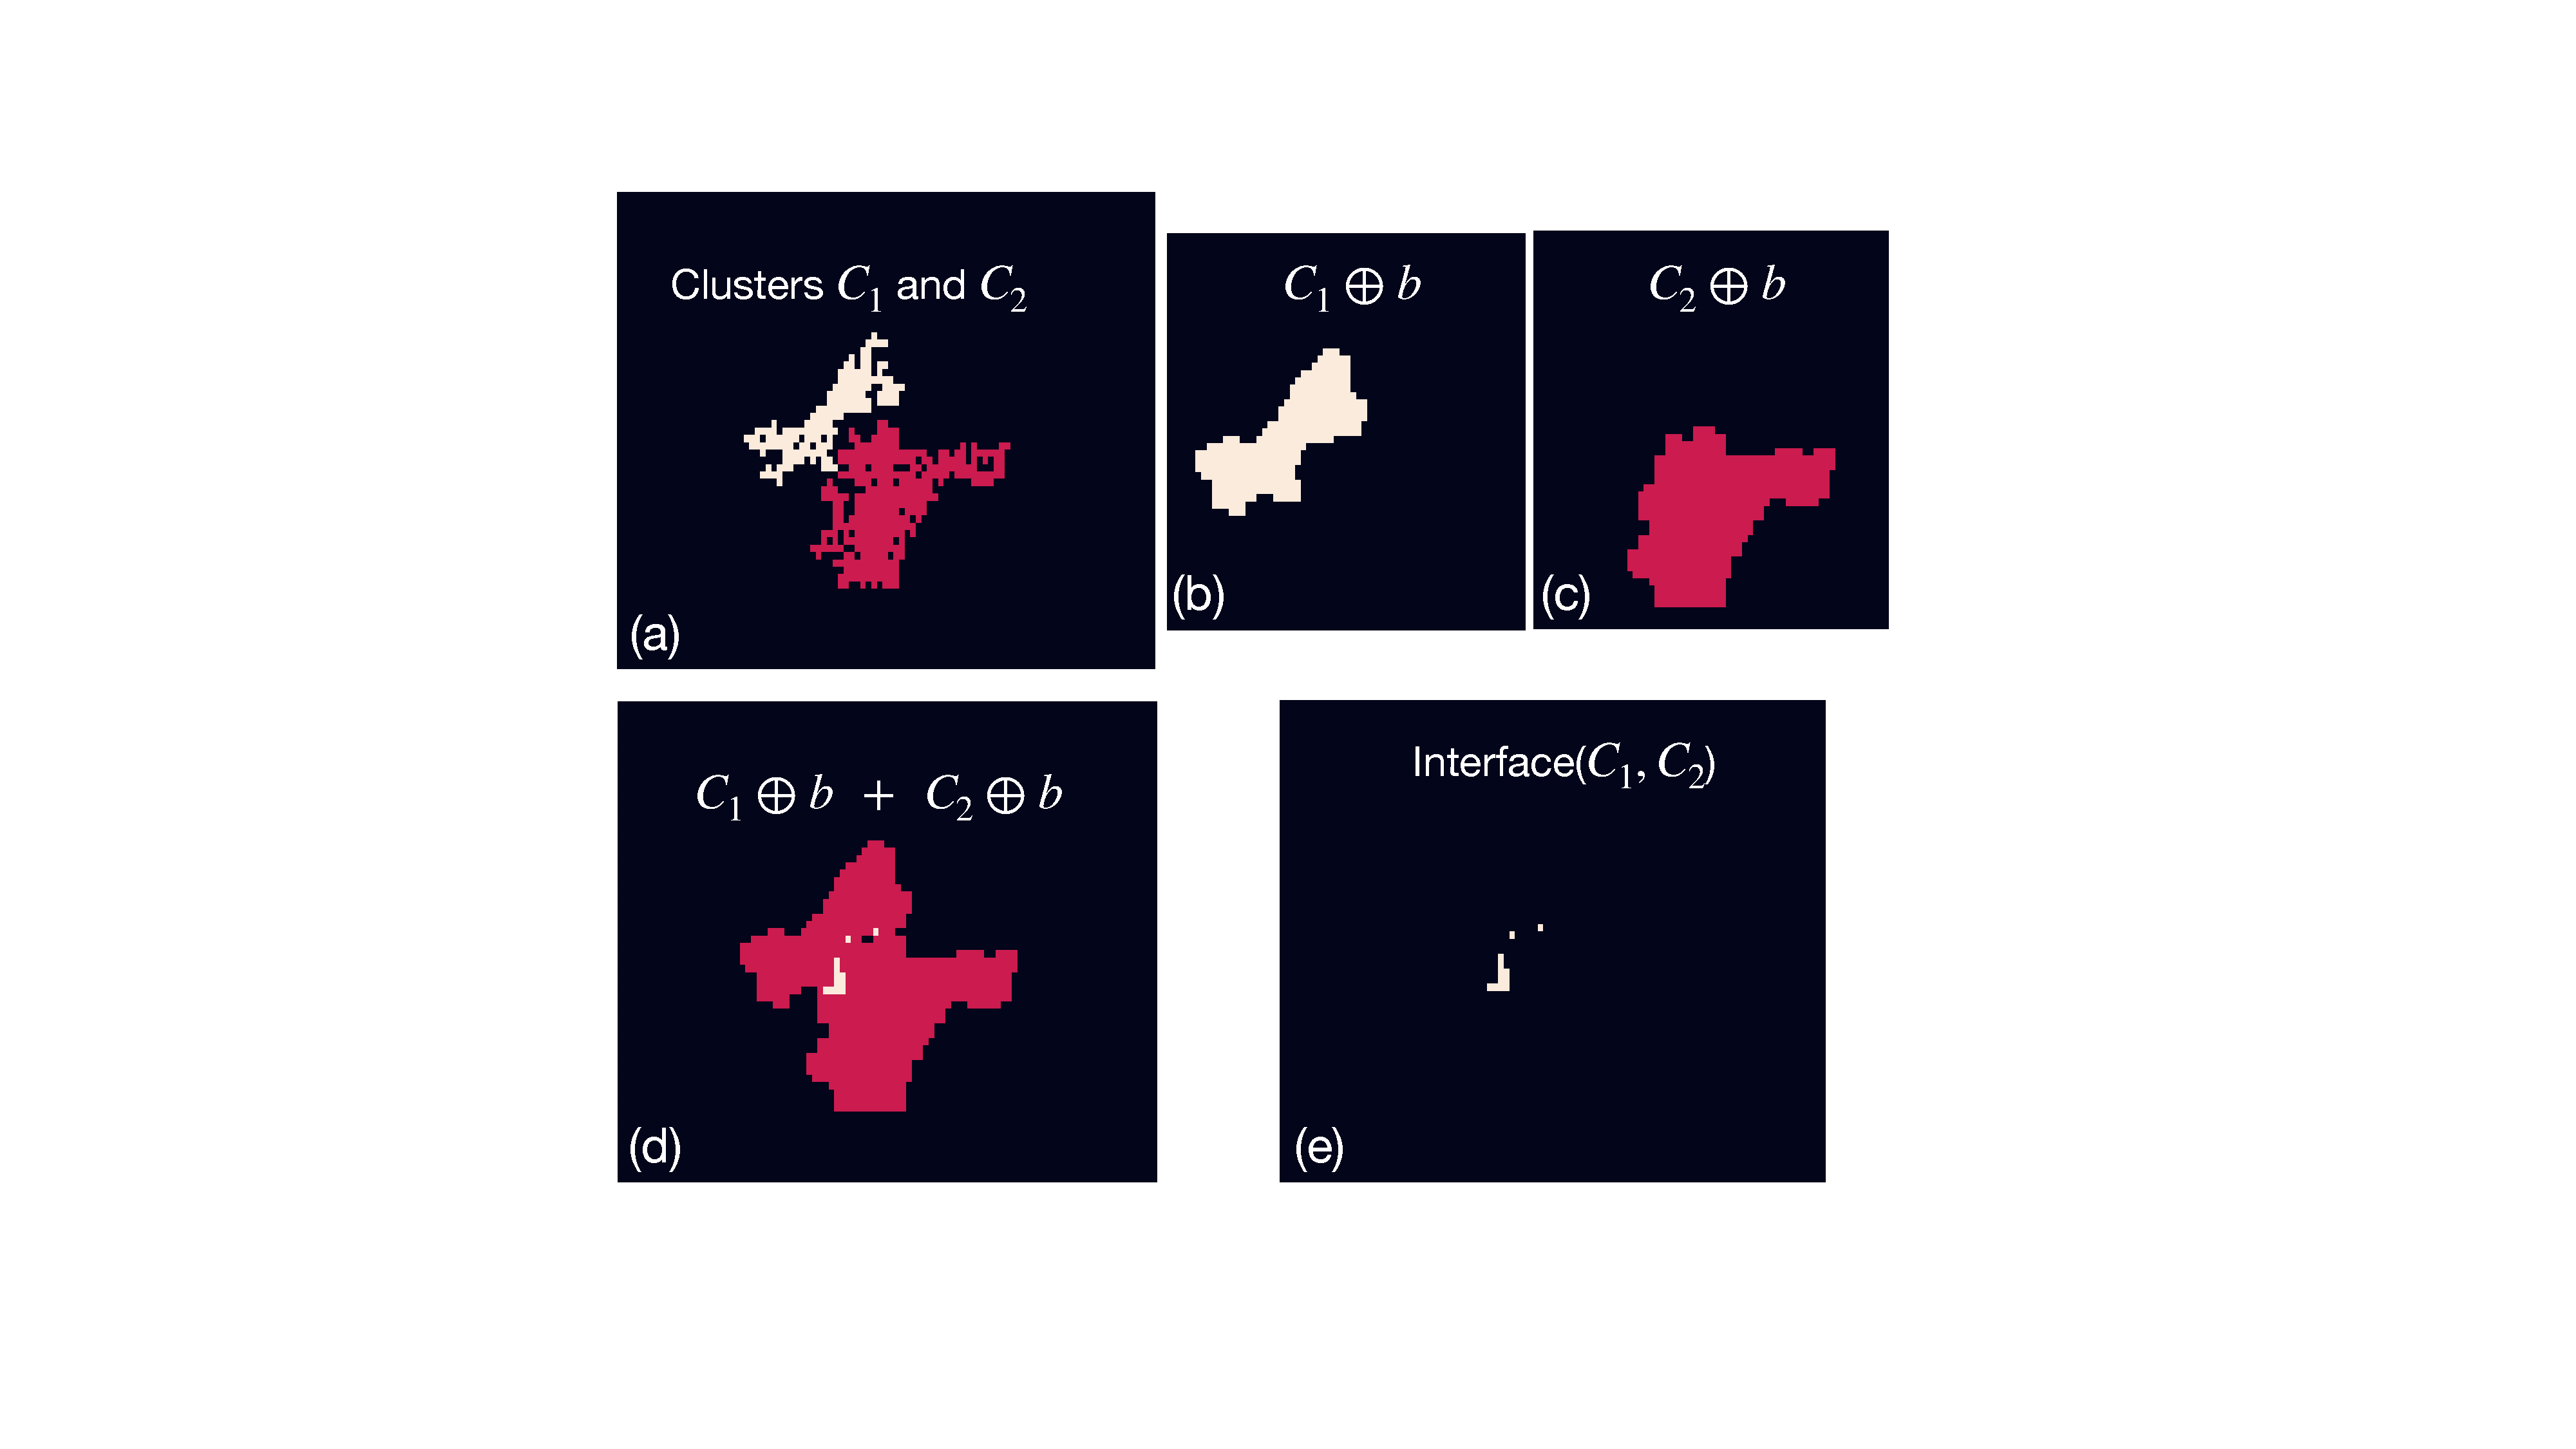
\includegraphics[scale=0.4]{appendix/figures/bd-interface.pdf}
    \caption{The binary dilator operator was used to help increase efficiency when identifying which susceptible patches bridge the gap between $\mathbf{C_1}$ and $\mathbf{C_2}$.
            Here, connectivity is defined with the Moore neighbour, $b$.}
    \label{fig:a-bd-interface}
\end{figure}
Below, the following steps detail a more efficient method:
\begin{enumerate}
    \item Prior to detecting a large rise in cluster size, label clusters $\mathbf{C_1}$ and $\mathbf{C_2}$, shown in Figure \ref{fig:a-bd-interface}(a).
    \item Perform a binary dilation on each cluster individually, shown in Figure \ref{fig:a-bd-interface}(b, c).
    \item Add both clusters arrays together in a pairwise fashion, shown in Figure \ref{fig:a-bd-interface}(d). 
    The interface between $\mathbf{C_1}$ and $\mathbf{C_2}$ now has the numerical value of $2$, easily singled out in Python (e.g. $\mathrm{np.where(Arr==2)}$), illustrated in Figure \ref{fig:a-bd-interface}(e).
    \item One or more of the interface patches must bridge the gap between $\mathbf{C_1}$ and $\mathbf{C_2}$. For each interface patch, test if a Moore neighbourhood
    falls within both $\mathbf{C_1}$ and $\mathbf{C_2}$; if so, it is a `\textit{connecting}' patch.
\end{enumerate}

\newpage

\begin{figure}
    \centering
    \includegraphics[scale=0.45]{appendix/Graphical_Abstract.pdf}
    \caption{A graphical abstract showing the end-to-end flow of 
    A) constructing a local-scale spatially-explicit model of pathogen dispersal 
    B) Scaling the small-scale epidemic model over a landscape 
    C) Identifying large susceptible clusters 
    D) Identifying areas for targeted landscape-level control.}
    \label{fig:my_label}
\end{figure}


